% -*- root: ../modelizacion.tex -*-
\section{Hoja 1}
\begin{problem}[1]
Una \textbf{fuerza central} es una fuerza que en $\overrightarrow{x}$ tiene módulo que sólo depende de $||\overrightarrow{x}||$. Por tanto $\overrightarrow F=m\cdot \overrightarrow a$ lleva a una ecuación del tipo
\[\overrightarrow x '' =g(||\overrightarrow x||)\overrightarrow x\]
Calcula la derivada de $\overrightarrow x\times \overrightarrow  x'$ (el momento angular) y deduce de ello que cada curva solución está contenida en un plano. Otra forma (más complicada) de proceder es probar directamente que la torsión de la curva es nula. Investiga este procedimiento usando la fŕomula de la torsión

\solution
	Definimos la fuerza central (la fuerza que va del origen hasta x) de la siguiente forma:$$\overrightarrow F = g(||\overrightarrow x||) \overrightarrow x$$

	Como $\overrightarrow F = m \cdot \overrightarrow a$ entonces $m\overrightarrow x'' = g(||\overrightarrow x||) \overrightarrow x$\\
	De esto último deducimos que $\overrightarrow x \times \overrightarrow x'' = \overrightarrow 0$ puesto que son vectores paralelos.

	Por lo tanto $\frac{\dif}{\dif t}(\overrightarrow x \times \overrightarrow x') = \overrightarrow x \times \overrightarrow x + \overrightarrow x \times \overrightarrow x '' = \overrightarrow 0 + \overrightarrow 0.$

	Y con esto ya tenemos que $\overrightarrow x $ está en un plano ya que:

	$$\overrightarrow x \times \overrightarrow x' = \overrightarrow V_0 \text{ que es }
	cte \implies \overrightarrow V_0 \cdot \overrightarrow x = 0 \stackrel{V_0 \neq 0}{\implies} \overrightarrow x \text{está en un plano}$$
	¿Qué ocurriría con $V_0 = 0$?

	$x'$ y $x$ serían paralelos, es decir, la velocidad iría en la dirección de x $\implies$ $\overrightarrow x$ está en una recta.

	La explicación de la última implicación se deja como ejercicio.

	Otra forma de ver que $\overrightarrow x$ está en un plano es utilizando la torsión:

	Definimos la curva
	\[t \mapsto \overrightarrow{x(t)}\]
	y la torsión
	\[T = \frac{(\overrightarrow x' \times \overrightarrow x'') \cdot \overrightarrow x'''}{||\overrightarrow x' \times \overrightarrow x ''||}\]

	Por la fórmula de la $\overrightarrow F$ puesdo escribir:
	$$\overrightarrow x'' = \frac{1}{m} g(||\overrightarrow x||)\overrightarrow x $$

	Y si dervivamos:

	$$\overrightarrow x''' = \frac{1}{m} g'(||\overrightarrow x||) \frac{\overrightarrow x \cdot \overrightarrow x'}{||\overrightarrow x||} \overrightarrow x + \frac{1}{m}g(||\overrightarrow x||)\overrightarrow x' = \frac{g'(||\overrightarrow x||)}{g(||\overrightarrow x||)}\cdot \frac{\overrightarrow x \cdot \overrightarrow x'}{||\overrightarrow x||} \overrightarrow x'' + \frac{1}{2}g(||\overrightarrow x||) \overrightarrow x''$$

	Con esto podemos ver que $\overrightarrow x'''$ es combinación lineal de $\overrightarrow x''$ y $\overrightarrow x'$ y por tanto:
	$$(\overrightarrow x' \times \overrightarrow x'' \times \overrightarrow x''') = det(\overrightarrow x', \overrightarrow x'',\overrightarrow x''') = 0 \stackrel{\implies}{\overrightarrow x' \times \overrightarrow x'' \neq 0} T = 0 \implies \text{curva plana}$$
\end{problem}

\begin{problem}[2]

La estación espacial internacional orbita a unos 400 km de la superficie dela Tierra. Calcula en qué proporción ha disminuido la fuerza de la gravedad a esa altura. ¿Cuánto pesaría una persona de 80kg a esa altura? ¿Por qué entonces las imágenesque nos llegan muestran astronautas y objetos flotando ingrávidos?

\solution
	Queremos ver el peso de una persona a 400 km de la Tierra

	Llamamos M a la masa de la tierra; m, al peso de una persona y R, al radio de la Tierra.

	Vemos la relación entre la fuerza que hay sobre la persona en la superficie de la Tierra y la fuerza a 400 km:

	$$\frac{\frac{GMm}{R^2}}{\frac{GMm}{(R + 400000 m)^2}} \implies \frac{(R + 4\cdot 10^5)^2}{R^2} = \left(\frac{67.8}{63.8}\right)^2$$

	Por lo tanto, si m = 80, el peso a 400 km sería:
	$$\frac{80}{\left(\frac{67.8}{63.8}\right)^2} = 70 .84 Kg$$

	\textbf{Pregunta del profesor:} Los astronautas están flotando alrededor de la Tierra por la fza.centrífuga. ¿Porqué no ocurre lo mismo en la superficie?
\end{problem}

\begin{problem}[3]
Prueba que la curva en polares $r(\theta)= \frac{a^{-1} \cdot b^2}{1 + e\cos\theta}$ siendo
\[ e = \frac{c}{a} = \sqrt{1 - \frac{b^2}{a^2}}\]
describe la elipse $\frac{x^2}{a^2} + \frac{y^2}{b^2} = 1$ cuando el origen de las coordenadas polares está en uno de los focos.

Prueba también que la curva en polares
\[r(\theta)=\frac{l}{1+e\cos(\theta)}\]
con $e \geq 0$ y $l>0$ constantes, describe una circunferencia si $e=0$, una elipse si $0<e<1$, una parábola si $e=1$ y una hipérbola si $e>1$.

\textbf{Indicación:} Escribe $r(1+e\cos(\theta)$ en cartesianas.

\solution

    Tenemos la elipse expresada en polares:$$r(\theta)= \frac{a^{-1} \cdot b^2}{1 + e\cos\theta} \text{  siendo  } e = \frac{c}{a} = \sqrt{1 - \frac{b^2}{a^2}}$$

    Y queremos llegar a: $$\frac{x^2}{a^2} + \frac{y^2}{b^2} = 1$$

    Esto es la elipse en cartesianas cuando el origen está en uno de sus focos. Como es lógico buscamos el cambio a cartesianas y para ello reescribimos la ecuación:

    $$ r + er\cos\theta = a^{-1} b^2 \text{ con }
    \begin{cases}
    r = \sqrt{x^2 + y^2}\\
    r\cos\theta = x\\
    \end{cases}$$

    Despejando y elevando al cuadrado en ambos lados obtenemos:
    \[(\sqrt{x^2 + y^2})^2 = (a^{-1}b^2 - ex)^2 \implies x^2 + y^2 = a^{-2} b^4 + e^2x^2 - 2a^{-1}b^2ex\]

    Agrupamos los términos:

    \[(1-e^2)x^2 + y^2 = a^{-2} b^4 - 2a^{-1}b^2ex\]


    Como $1-e^2 = \frac{b^2}{a^2}$ tenemos que

    $$\frac{x^2}{a^2}b^2 + y^2 = a^{-2} b^4 - 2a^{-1}b^2ex$$

    Viendo en la fórmula final el término $\frac{y^2}{b^2}$, dividimos por $b^2$ en ambos lados de la ecuación y completamos cuadrados para $x$ obteniendo:
    $$\frac{(x + a\cdot e)^2}{a^2} + \frac{y^2}{b^2} = 1$$

    Este resultado sería el que nos piden si $e$ vale cero ($a>0$), en cuyo caso es exactamente una circunferencia y el centro coincide con "los focos" tal y como se indica en el enunciado.
\end{problem}

\begin{problem}[4]
Sea $V$ el potencial de una fuerza $\overrightarrow F$, esto es $\overrightarrow F = -\nabla V$, que satisface div$\overrightarrow F = 0$. Demuestra que si $V$ es una función radial (sólo depende de la distancia al origen), entonces necesariamente $\overrightarrow F=K||\overrightarrow x||^{-3}\overrightarrow x$, como con la ley de gravitación universal

\solution
\textcolor{blue}{Hecho por De Juan. No fiarse al 100\%}

Podemos descomponer el potencial en una composición de 2 funciones:

$\appl{d}{ℝ^3}{ℝ}$, con $d(x,y,z) = \norm{\overrightarrow{x}}$.

$\appl{f}{ℝ}{ℝ}$.

Con esta construcción, para alguna $f$ tenemos $V(\vx) = f(d(\vx))$.

Si logramos demostrar que $f$ tiene que ser de la forma $f(x) = \frac{-KM}{x}$, ya tendremos el ejercicio hecho puesto que su gradiente nos daría una fuerza con fórmula como la indicada.

Ahora sólo hay que derivar con cuidado:

$$-\overrightarrow{F} = \grad V(\vx) = f'(d(\vx)) · \grad d(\vx) = f'\left(\norm{\vx}\right)\frac{1}{\norm{\vx}} \vx$$

\obs Hay que prestar especial atención al hecho de que al escribir $\vx$ hacemos referencia a un vector y no a una variable.

Vemos que $\appl{F}{ℝ^3}{ℝ^3}$. Calculamos la divergencia de $\overrightarrow{F}$

$$div \overrightarrow{F} = \frac{\partial{F}}{\partial{x}} + \frac{\partial{F}}{\partial{y}} + \frac{\partial{F}}{\partial{z}}
\overset{hip.}{=} 0$$


Basándonos en la expresión de la fuerza calculada anteriormente tenemos:

$$\frac{\partial{F(\vx)}}{\partial{x}} = \left(\underbrace{\dpa{f'(d(\vx))}{x}}_{(1)} · d(\vx) - f'(d(\vx))\dpa{d(\vx)}{x} \right)\frac{x}{(d(\vx))^2} + \frac{f'(d(\vx))}{d(\vx)}$$

$(1) = \dpa{d(\vx)}{x} · f''(d(\vx))$ por la regla de la cadena.

Simplificando y utilizando el cálculo anterior, obtenemos:

$$\dpa{F(\vx)}{x} = \frac{x^2}{(d(\vx))^3}\left(f''(d(\vx)) d(\vx) - f'(d(\vx))\right) + \frac{f'(\vx)}{d(\vx)}$$

El cálculo es análogo para las derivadas respecto de $y,z$, con lo que la divergencia queda:

$$div \overrightarrow{F} = \left(f''(d(\vx)) d(\vx) - f'(d(\vx))\right) \cdot \frac{x^2 + y^2 + z^2}{(d(\vx))^3} + \frac{3f'(d(\vx))}{d(\vx)}$$

Tomamos $d(\vx) = r$ y utilizamos $x^2+y^2+z^2 = \left(\sqrt{x^2+y^2+z^2}\right)^2 = d(\vx)^2$

$$ div \overrightarrow{F} = 0 = \left((f''(r)r - f'(r)) + 3f'(r)\right) \frac{1}{r} = 0 \dimplies r f''(r) = -2 f'(r)$$

Hemos llegado a una EDO cuya solución es $g(x) = \frac{k}{x}$, porque:

$$g(x) = \frac{k}{x} \implies g'(x) = \frac{-k}{x^2} \implies g''(x) = \frac{2k}{x^3}$$

Vemos que $x g''(x) = x\frac{2K}{x^3} = \frac{2K}{x^2} = -2 \frac{-K}{x^2} = -2 g'(x)$ que es la EDO que teníamos.

Por tanto ya tenemos el ejercicio resuleto, pues la $f$ obtenida coincide exactamente con lo que esperábamos obtener. Veamos por que está $f$ garantiza la fórmula para la fuerza que indica el enunciado.
$$V(\vx) = f(d(\vx)) = \frac{K}{d(\vx)} = \frac{K}{\norm{\vx}}$$

Y para hallar la $\overrightarrow{F}$, utilizamos $$\overrightarrow{F} = - \grad V = -K\left(\frac{-x}{\norm{\vx}^{3}},\frac{-y}{\norm{\vx}^{3}},\frac{-z}{\norm{\vx}^{3}} \right)$$

Y reescribimos : $$\overrightarrow{F} = - \grad V = \frac{K}{\norm{\vx}^3} \vx$$

\end{problem}

\begin{problem}[5]
Explica por qué en el punto más cercano al Sol de la órbita de una planeta, digamos a distancia $r_p$, la velocidad $v_p$ debe cumplir $v_p=r_p\theta'$. Recuerda que en el movimiento de un planeta $h=r^2\theta'$ es constante y que $a(1-e^2)=h^2/GM$ con $a$ el semieje mayor y  $e$ la excentricidad. Deduce de todo ello que $v_p=br^{-1}_p\sqrt{GM/a}$

\solution
Para probar que $v_p=r_p\dot{\theta}$ recordamos que estamos tomando $v_p = ||\overrightarrow v||_p$.

Cogemos la fórmula general de $v$ : $$ v = ||(\dot{x}, \dot{y})|| \implies v= \sqrt{\dot{x}^2 + \dot{y}^2}$$
Hacemos el cambio de variables
$\begin{cases}
x = r\cos\theta\\
y = r\sin\theta
\end{cases}$ de forma que
$$v = \sqrt{\dot{r}^2 + r^2\dot{\theta}^2}$$
Como en el punto más cercano al sol la distancia alcanza un mínimo $\implies \dot r = 0$, entonces
$$v= r\dot{\theta} \implies v_p = r_p\dot{\theta}$$

Ahora vamos a deducir:
\[v_p = \frac{b}{r_p}\cdot \sqrt{\frac{GM}{a}}\]

Por el enunciado sabemos que
$$v_p = \frac{h}{r_p} = \frac{\sqrt{GMa(1-e^2)}}{r_p}$$
Solo nos queda probar que $\sqrt{a(1-e^2)}= \frac{b}{\sqrt{a}}$, o l que es lo mismo
$$a(1-e^2) = \frac{b^2}{a}$$
Utilizamos la relación de la excentricidad (e) con los semiejes (a,b).

Sabemos que $e = \frac{c}{a}$, siendo c la distancia focal $\implies c= \sqrt{a^2-b^2}$ entonces $e = \frac{\sqrt{a^2 - b^2}}{a}$.

Sustituyendo:
$$a(1-e^2) = \frac{b^2}{a} \implies a(1-\frac{a^2 - b^2}{a^2}) = \frac{b^2}{a}$$
Vemos que es cierto, por lo tanto $v_p = \frac{b}{r_p}\cdot \sqrt{\frac{GM}{a}}$
%Esto lo comento por que creo que no vale para nada, pero me da pena tirarlo por si acaso
%Por el principio básico de la mecánica (principio de Hamilton) sabemos que la trayectoria del sistema da un extremo de
%\[\int_{t_0}^T L = \int_{t_0}^T E_{cinetica}-E_{potencial} = \int_{t_0}^T \frac{1}{2}mv^2-\frac{GMm}{r}\]
%Sabiendo que la velocidad es la derivada de la posición y que las órbitas son planas podemos escribir:
%\[\int_{t_0}^T L = \int_{t_0}^T \frac{1}{2}m\left(\dot{x}^2+\dot{y}^2\right)-\frac{GMm}{\sqrt{x^2+y^2}}\]
%Puesto que no depende de $t$ tenemos que la energía es constante. Es decir:
%\[E = \dot{x}\frac{\partial L}{\partial \dot{x}}+\dot{y}\frac{\partial L}{\partial \dot{y}}-\frac{1}{2}m\left(\dot{x}^2+\dot{y}^2\right)-\frac{GMm}{\sqrt{x^2+y^2}} = cte\]
%Vamos a trabajar esta ecaución a fin de llegar al resultado buscado:
%\[\dot{x}\dot{x}'+\dot{y}\dot{y}'-\frac{1}{2}\left(\dot{x}^2+\dot{y}^2\right)-\frac{GM}{\sqrt{x^2+y^2}} = cte\]
\end{problem}

\begin{problem}[6]
Prueba que si el semieje mayor de la elipse de un planeta es $a$ entonces su velocidad cuando está a distancia $r$ del Sol es $\sqrt{2GM/r-GM/a}$.

\textbf{Indicación:} Utiliza el problema anterior y la conservación de la energía.
\solution
\textbf{Idea:} En $v_p = \frac{b}{r_p}\cdot \sqrt{\frac{GM}{a}}$ (ejercicio anterior) hay información redundante, ya que $b,a\text{ y } r_p$ están relacionadas, no son independientes.

La conservación de la energía me dice que
$$\frac{1}{2}m v^2 - \frac{GMm}{r} \text{ es cte}$$

Como tengo la velocidad en un punto ($v_p$), me queda
$$\frac{1}{2} v^2 - \frac{GM}{r} = \frac{1}{2} v_p^2 - \frac{GM}{r}$$
Entonces
$$v = \sqrt{\frac{2GM}{r} + v_p^2 - \frac{2GM}{r_p}}$$
¿Cómo simplifico esto? mirando lo que queremos demostrar sólo queda probar que:
$$\frac{2GM}{r_p} - v_p^2 = \frac{GM}{a}$$
Sustituimos $v_p$ por lo que teníamos en el ejercicio anterior:
$$\frac{2GM}{r_p} - v_p^2 =\frac{2GM}{r_p} -\frac{GMb^2}{ar_p^2} = \frac{GM}{r_p}\left(2-\frac{b^2}{a r_p}\right) $$
Para que la expresión se parezca más a lo que queremos demostrar pensamos qué relación hay entre $r_p$ y a.


Como $e = \frac{c}{a}$ y $r_p = a-c$, sustituyendo:$$\frac{GM}{a(1-e)} \cdot \left(2-\frac{b^2}{a^2(1 - e)}\right)$$

Para terminar bastaría comprobar que:
$$\frac{1}{(1-e)} \cdot (2- \frac{b^2}{a^2(1-e)}) = 1$$

Es fácil usando las siguientes propiedades:
$$e^2 = \frac{c^2}{a^2} = 1-\frac{b^2}{a^2} \implies b^2 = a^2(1-e^2)$$

Finalmente
$$\frac{1}{1-e} \cdot \left(2 - \frac{1 - e^2}{1 - e}\right) = \frac{1}{1-e} \cdot (2-(1 + e)) = 1$$

Por tanto queda demostrado que
$$\frac{2GM}{r_p} - v_p^2 = \frac{GM}{a}$$

Y ya tenemos sustituyendo en la ecuación inicial que
\[v=\sqrt{\frac{2GM}{r}- \frac{GM}{a}}\]
\end{problem}

\begin{problem}[7]
El cometa Halley tiene distancias máxima y mínima al Sol dadas por $5.25\cdot 10^{12} m$ y por $8.77\cdot10^{10}$ m, respectivamente. Calcula la fórmula de su elipse en coordenadas cartesianas, su valor de $r^2\theta'$ y sus velocidades máxima y mínima.

\solution

\textbf{Solución de clase}

$$ \frac{(x+c)^2}{a^2} + \frac{y^2}{b^2} =  1 \;\;\;\; c = a e $$

$$ \begin{cases}
		a + (1+e) = 5.25 * 10^{12} \\
		a(1-e) = 8.77 * 10^{10}
	\end{cases} \} \Rightarrow \begin{cases}
		a = 2.67 * 10^{12} \\
		e = 0.967
	\end{cases}$$

	Con esto calculamos $c = a e = 2.58 * 10^{12}$ y $b = 6.80 * 10^{11}$

\textbf{b)} clase (ver ej. 5)

$$ \frac{h^2}{GM} = a(1- e^2) \;\;\; h = r^2 \theta' $$
$$ h = r^2 \theta' = \sqrt{GMa(1 - e^2)} = 5.53 * 10^{25} $$

\textbf{c)} $v_{\text{max}}$  $ v_{\text{min}}$

Hay que tener en cuenta que la velocidad máxima se alcanza en el perihelio (punto de la órbita con distancia más corta) y la mínima en el afelio (punto opesto al perihelio).

$$ v_{\text{max}} = \sqrt{\frac{2GM}{a(1-e)} - \frac{GM}{a}} =^{\text{a)}} 5.45 * 10^4 m/s $$

$$ v_{\text{min}} = \sqrt{\frac{2GM}{a(1+e)} - \frac{GM}{a}} =^{\text{a)}} 9.14 * 10^2 m/s $$

\end{problem}

\begin{problem}[8]
La excentricidad de la órbita de la Tierra es aproximadamente $e=0.017$. Si en un libro de texto vemos la órbita dibujada con un eje mayor de $20cm$, ¿cuánto debería medir el eje menor?. Suponemos, consecuentemente, la órbita de la Tierra circular. Si en una galaxia lejana hay un planeta hermano de la Tierra con la misma órbita pero recorrida sólo en tres meses, ¿qué relación hay entre la masa de su estrella y la de nuestro Sol?

\solution
\textcolor{blue}{Hecho por Pedro. No fiarse al 100\%}

Puesto que la excentricidad sea calcula como $e=c/a$ siendo $c$ la mitad de la distancia focal y $a$ el semieje mayor de la elipse, podemos deducir fácilmente que la semidistancia focal es
\[c= 0.17cm\]
y sabiendo ahora que $a^2 = c^2+b^2$, con $b$ es semieje menor, podemos despejar y obtener que
\[b = \sqrt{a^2-c^2}=\sqrt{399.9711} = 19.99921 cm\]

Puesto que la diferencia entre los semiejes de la elipse es mínima, tiene sentido considerar la órbita como circular.

Ya sabemos que podemos calcular el área de la órbita de un planeta como
\[A = \frac{1}{2}h T \text{ siendo } h = cte \text{ dependiente del planeta }\]
Puesto que nuestro nuevo planeta y la Tierra tienen la misma órbita, aunque la recorran a distintas velocidades, su área será la misma.

Por tanto, puesto que nuestro nuevo planeta tiene un período 4 veces menor, tenemos que $h_N=h_T \cdot 4$.

Si recordamos el ejercicio 1.5 ya vimos que
\[a(1-e^2)=\frac{h^2}{GM}\]
puesto que $a,e,G$ no cambian al pasar de estudiar la Tierra a este nuevo planeta, tenemos que
\[h_N=\sqrt{a(1-e^2)GM_{NS}}=4h_T=\sqrt{16a(1-e^2)GM} \implies \sqrt{M_{NS}}=\sqrt{16M}\]
es decir, el nuevo Sol tendrá 16 veces la masa del nuestro.

\end{problem}

\begin{problem}[9]
Sabiendo que $GM=3.99\cdot 10^{14}m^3s^{-2}$ con $M$ la masa de la Tierra, calcula a qué distancia de su superficie orbitan los satélites goestacionarios: los que están siempre sobre el mismo punto geográfico porque giran a al par que la Tierra, una vez cada 24 horas.
\solution

La 3ª ley de kepler nos da una relación entre la distancia y el periodo orbital. En concreto:
\[\frac{T^2}{R^3} = \text{ cte } = \frac{4\pi^2}{GM} \]

Para que sea geostacionario $\rightarrow T = 24h = 24 * 3600 s$.

$$ R = \left( \frac{GMT^2}{4\pi^2} \right)^{1/3} = 4.23 * 10^7 m $$

$$ R_{s} = R - \text{radio de la tierra} = 4.23 * 10^{7} - 6.38 * 10^{6} = 3.58 * 10^{7} m $$

Aproximadamente 35.000 Km


\end{problem}

\begin{problem}[10]
Usando la ley de Gauss, prueba que en un planeta esférico homogéneo hueco no hay gravedad en el interior.
\solution

\textcolor{blue}{Hecho por Pedro. No fiarse al 100\%}

Según la ley de Gauss la fuerza de la gravedad en un punto de una superficie será proporcional al flujo del campo gravitatorio a través de dicha superficie.

Una vez tomamos un punto en el interior del planeta hueco, consideramos la esfera que lo contiene y que, a su vez, se contiene dentro del planeta.

Para calcular la fuerza de la gravedad en ese punto (o en cualquiera de la esfera que hemos construido, pues todos comparten el mismo valor de gravedad) basta con calcular el flujo del campo gravitatorio en torno a la esfera.

Puesto que esta esfera está hueca y las líneas de campo vienen desde el infinito hasta la superficie del planeta, no hay líneas de campo dentro del planeta por lo que no hay líneas de campo que atraviesen nuestra esfera, por lo que no hay flujo y por tanto, por el teorema de Gauss, no habrá gravedad.
\end{problem}

\begin{problem}[11]
Newton resolvió el problema anterior con un bello argumento geométrico: Fijado un
punto interior se considera un doble cono que lo tiene como vértice. El cono corta a la superficie interior del planeta en dos regiones que cuando se reducen a tamaño infinitesimal ejercen la misma atracción. Intenta elaborar este argumento hasta que te suene convincente.

\solution

\end{problem}

\begin{problem}[12]
Utilizando las ecuaciones de Euler-Lagrange con coordenada generalizada la distancia desde el punto de partida, halla las ecauciones de movimiento de un objeto de masa $m$ que cae por un plano inclinado de ángulo α partiendo del reposo. La energía potencia gravitatoria es $mgy$ donde $g=9.8ms^{-2}$ e $y$ es la altura.

\solution
\textcolor{blue}{Hecho por Pedro. No fiarse al 100\%}

Tomemos nuestra variable $z(t)$ que define la distancia en línea recta desde el punto de partida hasta la posición actual de la masa.

El Lagrangiano sería:
\[\int_a^b L = \int_a^b E_c-E_p = \int_a^b \frac{1}{2} m \left(z'(t)\right)^2+mgz(t)\sin(α)\]
aplicando las ecuaciones de Euler-Lagrange llegamos a
\[\frac{\partial}{\partial t} mz'(t) = mg\sin(α)\]
de donde podemos deducir que
\[z'(t)=g\sin(α)t + C_1 \implies z(t)=\frac{1}{2}g \sin(α)t^2+C_1t+C_2\]
Así, la ecuación del movimiento de la partícula sería de la forma
\[\left(x(t),y(t)\right) = \left(x_0+\frac{1}{4}g\sen(2α)t^2+\cos(α)(C_1t+C_2),y_0-\frac{1}{2}g \sin^2(α)t^2 +\sin(α)(C_1t+C_2)\right)\]

\textcolor{green}{Corrección de clase}

Tenemos que
\[ L = T - V\]
Siendo $T$ la energía cinética y $V$ energía potencial.

Llamamos H a la altura y q la trayectoia del objeto 

\[ \frac{d}{dt} \cdot \frac{\partial L}{\partial \dot{q_i}} = \frac{\partial L}{\partial q_i}\]

Entonces escribimos
\[ x = q\cos \alpha \rightarrow \dot{x} \dot{q} \cos\alpha\]
\[ y =H - q\sin \alpha \rightarrow \dot{y} -\dot{q} \sin\alpha\]

Y ahora la energía potencial y cinética
\[ T = \frac{1}{2} m v^2 = \frac{1}{2} m (x^2 + y^2) = \frac{1}{2} m \dot{q}^2\]
\[ V = mg (H- q \sin\alpha)\]

Con esto calculamos L y con las ecuaciones de $\frac{d}{dt} \cdot \frac{\partial L}{\partial \dot{q_i}} = \frac{\partial L}{\partial q_i}$ llegamos a 
\[ m \ddot{q}^2 = mg\sin\alpha \implies \ddot{q}^2 = g \sin\alpha\]
\end{problem}

\begin{problem}[13]
Sea $G_α$ un giro en $\real^3$ de ángulo α alrededor de un eje dado por un vector unitario $\vn$ y sea $f(α)=G_α(\vx)$ para un $\vx\in \real^3$. Prueba que $f'(0)=\vn \times \vx$ y utiliza el teorema de Noether para deducir que si $L=\frac{1}{2}m||\vv||^2-V(||\vx||)$, entonces el momento angular $\vx \times m \vv$ se conserva.
\solution

\textcolor{blue}{Hecho por Pedro. No fiarse al 100\%}

La matriz de giro de α grados respecto al vector $\vn$ tiene la siguiente matriz:
\[\begin{bmatrix} \cos α +n_x^2 \left(1-\cos α\right) & n_x n_y \left(1-\cos α\right) - n_z \sin α & n_x n_z \left(1-\cos α\right) + n_y \sin α \\ n_y n_x \left(1-\cos α\right) + n_z \sin α & \cos α + n_y^2\left(1-\cos α\right) & n_y n_z \left(1-\cos α\right) - n_x \sin α \\ n_z n_x \left(1-\cos α\right) - n_y \sin α & n_z n_y \left(1-\cos α\right) + n_x \sin α & \cos α + n_z^2\left(1-\cos α\right)
\end{bmatrix}\]

Si ahora derivamos con respecto a α obtenemos:
\[\begin{bmatrix} -\sin α +n_x^2 \left(1+\sin α\right) & n_x n_y \left(1+\sin α\right) - n_z \cos α & n_x n_z \left(1+\sin α\right) + n_y \cos α \\ n_y n_x \left(1+\sin α\right) + n_z \cos α & -\sin α + n_y^2\left(1+\sin α\right) & n_y n_z \left(1+\sin α\right) - n_x \cos α \\ n_z n_x \left(1+\sin α\right) - n_y \cos α & n_z n_y \left(1+\sin α\right) + n_x \cos α & -\sin α + n_z^2\left(1 +\sin α\right)
\end{bmatrix}\]

y al evaluar esta derivada en α=0 tenemos:
\[\begin{bmatrix} n_x^2 & n_x n_y - n_z & n_xn_z + n_y \\
n_y n_x+ n_z & n_y^2 & n_y n_z - n_x \\
n_z n_x - n_y 1 & n_z n_y + n_x &  n_z^2
\end{bmatrix}\]

Ahora nos fijamos en que calcular $f'(0)$ es lo mismo que derivar la matriz con respecto a α, evaluar en 0 y multiplicar por $\vx$. Por tanto, para calcular el valor pedido sólo hace falta multiplicar por $\vx$

\textcolor{blue}{TO BE CONTINUED ...}

No se cómo puñetas se acaba esta parte.

Vamos a por la segunda parte. Para poder empelar el teorema de Noeter debemos encontrar las invariantes del Lagrangiano. En este ejemplo, podemos ver que si aplicamos la transformación $(x,y,z) \to (x\cos h-y \sin h, x \sin h +y \cos h, z)$ el Lagrangiano conserva su valor\footnote{Estamos aplicando un giro a todo el sistema}

Si escribimos el lagrangiano con la notación habitual vista en calse y desarrollada por Newton tenemos:
\[L=\frac{1}{2}m(\dot x ^2+\dot y^2+\dot z^2)-\frac{Gmm}{\sqrt{x^2+y^2+z^2}}\]
Si aplicamos ahora el teorema tenemos:
\[0 = \frac{\partial L }{\partial h} = \frac{\partial}{\partial t}\left(\frac{1}{2}m\left(2 \dot x\cdot (-x \sin h -y \cos h) + 2 \dot y\cdot (x \cos h -y \sin h) +2 \dot z \cdot 0\right)\right)\]

Evaluando en $h=0$ tenemos:
\[m (-\dot x y, \dot y x, 0) = \text{ cte}\]

que coincide con la tercera componente del producto $m \vx \times \vv$. Repitiendo ahora este proceso con giros en torno a los otros ejes (el giro que hemos cogido rotaba en torno al eje $Z$) obtendremos las demás componentes.

\textcolor{red}{Guille: Propuesta de resolución más simple}

\begin{figure}[hbtp]
\centering
\inputtikz{hoja1_ej13}
\caption{Giro del vector en el plano}
\label{figHoja1Ej13}
\end{figure}

Podemos suponer sin pérdida de generalidad que $\vec{n} = (0,0,1)$. Ya nos han asegurado que el vector normal al plano es unitario, por lo que si el vector no es el unitario en la dirección de $Z$ simplemente tenemos que hacer giros y traslaciones que conservan ángulos y distancias. Es decir, que nos basta con considerar este caso para estudiar el problema. Por la misma razón, podemos suponer también que $\vx = \md{\vx} · (1,0,0)$ (un vector en la dirección del eje $X$) y llamaremos $r = \md{\vx}$ por simplicidad.

Con estas simplificaciones nos encontramos en las condiciones de la figura \ref{figHoja1Ej13}. Es fácil ver que, de esta forma, se puede expresar $f(α)$ como \[ f(α) = (r \cos α, r \sin α, 0) \], que derivando nos da $f'(α) = (-r \sin α, r \cos α, 0)$.

Por otra parte, si hallamos el producto vectorial vemos que $\vn × f(α) = (-r \sin α, r \cos α, 0)$, exactamente lo mismo que antes. Concuerda con el dibujo ya que la dirección de giro tangente a la circunferencia es la misma dirección que la del producto vectorial.

La segunda parte se haría como ha propuesto Pedro, con la ventaja de que así probablemente saldría mucho más sencillo, aprovechando que el teorema de Noether nos dice que el Lagrangiano se conserva en cambios de coordenadas o algo así.

\end{problem}


\begin{problem}[14]
Sabiendo que entre las superficies de revolución cuyos bordes son $\{x^2+y^2 = 4, \ z= \pm 1\}$ hay una de área mínima, prueba que es $\sqrt{x^2+y^2}=C\cosh(z/C)$ con $C \approx 1.69$

\textbf{Indicación:} Recuerda (o demuestra) que si la gráfica de $y=y(x)$, $a\leq x \leq b$ gira alrededor del eje $X$ el área de la superficie resultante es $2\pi \int_a^by\sqrt{1+(y')^2}dx$. Después aplica el cálculo de variaciones preferentemente valiéndote de la energía.
\solution

Este problema es equivalente a hallar la superficie generada por dos aros con jabón que une ambos perímetros. La membrana generada intentará alcanzar un área mínima para tener tensión superficial mínima también.

La superficie buscada, en cilíndricas es $r = r(z)$ (Las superficies de revolución son unión de circunferencias, basta tener el radio a lo largo del eje).

El área de una superficie de revolución se calcula con la fórmula:
\[ 2\pi \int r\sqrt{1+(r')^2}dz  \]

Para minimizar usamos las ecuaciones de Euler-Lagrange \ref{ecuaciones-euler-lagrange}:

$$ L (r, r') = r \sqrt{1+(r')^2} r = r(z)$$

$$\frac{d}{dz} \left( \frac{\partial L}{\partial r'} \right) = \frac{\partial L}{\partial r} $$

Sale pero la ecuación es un poco fea. Así que probamos de otra manera (conservanción de la energía):

Como ya hemos visto muchas veces junto al teorema de Lagrange, la energía:
\[E = r' \frac{\partial L}{\partial r'} - L \]
se conserva (es cte.). Por tanto

$$ E = r' r \frac{r'}{\sqrt{1 + (r')^2}} - r \sqrt{1 + (r')^2} =^{\text{milagro}} \frac{-r}{\sqrt{1 + (r')^2}} $$
$$ \Rightarrow r' = \sqrt{\left( \frac{r}{E} \right)^2 - 1}  $$

Y resulta que:
$$ \int \frac{dr}{\sqrt{\left( \frac{r}{E} \right)^2 - 1}} = \int dz $$.

$$ E \text{arc}\cosh{\frac{r}{E}} = z + \text{cte.} $$

$$ r = E \cosh{\frac{z}{E} + \text{cte.}} $$

Adicionalmente, para que pase por las circunferencias:

$$ r(1) = 2 \;\;\;\; r(-1) = 2 \;\;\;\; \text{cte} = 0 $$

$$ 2 = E \cosh{\frac{1}{E}} \Rightarrow^{\text{aproximado con el ordenador}} E = 1.69 $$


La constante debe ser nula

\end{problem}

\begin{problem}[15]
Para lagrangianos unidimensionales $L(x, \dot{x})$, prueba directamente, únicamente con diversas formas de la regla de la cadena, que las ecuaciones de Euler-Lagrange son invariantes por cambios de variable $y = y(x)$.

\solution
\textcolor{blue}{Hecho por Pedro y Edu. No fiarse al 100\%}

%Con el lagrangiano dado, las ecuaciones de Euler-Lagrange quedan de la forma:
%\[\frac{d}{dt}\left(\frac{\partial L}{\partial \dot x}\right) = \frac{\partial L}{\partial x}\]
%
%Si ahora tuviéramos el Lagrangiano L(y(x), $\dot y(x)$) y calculamos las ecuaciones de Euler-Lagrange tendríamos:
%\[\frac{d}{dt}\left(\frac{\partial L}{\partial \dot y} \frac{d\dot y}{d\dot x}\right) = \frac{\partial L}{\partial y}\frac{dy}{dx} \implies\footnote{y(x) $\implies \dot y = \dot x \dot y(x)$} \frac{d}{dt}\left(\frac{\partial L}{\partial \dot y} \dot y\right) = \frac{\partial L}{\partial y}\dot y \]
%aplicando una vez más la regla de la cadena tenemos:
%\[\frac{d}{dt}\left(\frac{\partial L}{\partial \dot y} \right) \cdot \dot y + \frac{\partial L}{\partial \dot y} \frac{d \dot y}{dt}=  \frac{\partial L}{\partial y}\dot y\]
%
%Esta ecuación sería idéntica a la inicial, con lo que demostraríamos que las ecuaciones de Euler-Lagrange son invariantes por cambio de variable, si lográsemos probar que:
%\[\frac{\partial L}{\partial \dot y} \frac{d \dot y}{dt}=0\]
%lo cual es cierto puesto que $\dot y$ depende de $x$ y no de $t$ por lo que
%\[\frac{d\dot y}{dt}=0\footnote{triplazo, pero por ahí van los tiros}\]
%
Según el cambio de variable que se indica en el enunciado, tenemos la siguiente relación:
\[\bar{L}(y,\dot y)=L(x, \dot x) \text{ con } y=y(x)\]

Como nos hará falta a continuación, vamos a ver que
\[\dot y = \frac{\partial}{\partial t} y(x(t))=\frac{\partial y}{\partial x} \frac{\partial x}{\partial t} = \frac{\partial y}{\partial x}  \dot x \]

Vamos a escribir ahora las ecuaciones de Euler-Lagrange con $\bar{L}$ con las variables $y, \dot y$ y veremos que son equivalentes a las obtenidas trabajando con $L$ con las variables $x, \dot x$.

\[\frac{\partial}{\partial t}\left(\frac{\partial \bar{L}}{\partial \dot x} \right)=\frac{\partial \bar{L}}{\partial x} \implies \frac{\partial}{\partial t} \left( \frac{\partial \bar{L}}{\partial \dot y}\frac{\partial y}{\partial x}\right) = \frac{\partial \bar{L}}{\partial y}\frac{\partial y}{\partial x}+\frac{\partial L}{\partial \dot y}\frac{\partial^2 y}{\partial^2 x}\dot x \implies \]

aplicando la regla de la cadena a la izquierda de la igualdad llegamos a:
\[\implies \frac{\partial}{\partial t} \left( \frac{\partial L}{\partial \dot y}\right)\frac{\partial y}{\partial x} + \frac{\partial L}{\partial \dot y}\frac{\partial}{\partial t} \left( \frac{\partial y}{\partial x}\right) = \frac{\partial \bar{L}}{\partial y}\frac{\partial y}{\partial x}+\frac{\partial L}{\partial \dot y}\frac{\partial^2 y}{\partial^2 x}\dot x\]

Si probamos que
\[\frac{\partial L}{\partial \dot y}\frac{\partial}{\partial t} \left( \frac{\partial y}{\partial x}\right) = \frac{\partial L}{\partial \dot y}\frac{\partial^2 y}{\partial^2 x}\dot x\]
podremos simplificar y obtendremos el resultado esperado. Vamos a ello.

\[\frac{\partial L}{\partial \dot y}\frac{\partial}{\partial t} \left( \frac{\partial y}{\partial x}\right) = \frac{\partial L}{\partial \dot y}\frac{\partial}{\partial t} \left( \frac{\partial y}{\partial x}\right) = \frac{\partial L}{\partial \dot y}\frac{\partial^2 y}{\partial^2 x}\frac{\partial x}{\partial t}\]
con lo que ya lo tenemos.

\end{problem}

\section{Hoja 2}

\begin{problem}[1]
	Una cadena de Markov con tres estados, {1, 2, 3}, tiene probabilidades de transición
	$p_{ij} = i/10$ para $1 ≤ i ≤ 3$ y $j ∈ {1, 2}$. Calcula $\prob{X1 = X2 = 2|X0 = 1}$.

	\solution
	Las probabilidades de transición son por definición:
	$$P_{ij} = \prob{X_{n+1} = j | X_n = i}$$

	Por Bayes sabemos que:
	$$\prob{B\cap C|A} = \prob{B|A} \cdot \prob{C|A\cap B}$$

	Siendo
	\begin{itemize}
		\item 	$\prob{B\cap C|A} = \frac{\prob{B\cap C \cap A}}{\prob{A}}$
		\item  $ \prob{B|A} = \frac{\prob{B\cap A}}{\prob{A}}$
		\item  $\prob{C|A\cap B}= \frac{\prob{C\cap A \cap B}}{\prob{A\cap B}}$
	\end{itemize}

	Llamamos $B={X_1 = 2}$ y $C={X_2 = 2}$ de forma que:
	\[\prob{X_1 = X_2 = 2|X_0 = 1} = \prob{X_1 = 2 \cap X_2 = 2|X_0 = 1} =\]
	\[= \prob{X_1=2|X_0=1} \cdot \prob{X_2 =2 |X_0 = 1 \cap X_1 =2}\]

	Vemos que $\prob{X_1=2|X_0=1}$ es la probabilidad de transición $p_{12}$

	La parte de $\prob{X_2 =2 |X_0 = 1 \cap X_1 =2}$ se puede escribir como $\prob{X_2 =2 | X_1 =2} = p_{22}$ ya que por definición, una cadena de Markov sólo depende del suceso anterior.

	Por lo que nos queda que
	$$\prob{X1 = X2 = 2|X0 = 1} = p_{12} \cdot p_{22} = \frac{1}{10} \cdot \frac{2}{10} = \frac{1}{50}$$
\end{problem}




\begin{problem}[2]
	Considera la cadena de Markov con cuatro estados y con probabilidades de transición
	$p_{12} = p_{24} = p_{43} = p_{32} = 1$. Halla para qué distribuciones iniciales existe una distribución
	límite.
	\solution
	Primero construimos la matriz de transición:

	$P = \left(\begin{matrix}
	0&1&0&0\\0&0&0&1\\0&1&0&0\\0&0&1&0\\
	\end{matrix}\right)$

	Podríamos utilizar Jordan para calcular el límite, pero en este caso, al haber tantos ceros, es más fácil hacer las operaciones.

	Cogemos una distribución inicial

	$(\prod_0)= (x,y,z,t)$

	que por ser distribución de probabilidad tiene $x+y+z+t=1$

	Ahora tenemos que ver si existe $\lim (\prod_0) P^n $

	Haciendo $(\prod_0) \rightarrow (\prod_0)\cdot P \rightarrow (\prod_2) = (\prod_1) \cdot P = (\prod_0)\cdot P^2 \rightarrow . . . . $

	Nos queda que
	$$(x,y,z,t) \rightarrow (0,x+z,t,y) \rightarrow (0,t,y,x + z)\rightarrow(0,y,x+z,t) \rightarrow . . . $$
	Vemos que siempre va a oscilar de la manera $(0,a,b,c) \rightarrow (0,b,c,a)$

	Por lo tanto la única posibilidad de que converjan es que a,b,c sean iguales. Por lo tanto todas las distribuciones iniciales que estoy buscando tienen que cumplir.

	$\begin{cases}
		 x + y + z + t = 1\\
		 x+z=t=y
	\end{cases} \implies (\prod_0) = (x,\frac{1}{3}, \frac{1}{3},\frac{1}{3} -x)$ con $0 \leq x \leq \frac{1}{3}$

	Y la distribución límite sería:
	$$\left(\prod_n\right) = \left(0, \frac{1}{3}, \frac{1}{3}, \frac{1}{3}\right)$$
\end{problem}

\begin{problem}[3]
	Lanzamos una moneda al aire y consideramos la variable aleatoria $X_n$ que da el número
	de caras en las tiradas n y n − 1. ¿Es $\{X_n\}^{\infty}_{n=1}$ una cadena de Markov?
	\solution

	Para saber si es una cadena de Markov lo que tenemos que ver es si el resultado del caso $n$ depende de $n-1$, $n-2$, $n-3$...(caso en el que \textbf{no} sería Markov) o si solo depende de $n$ y $n-1$

	En otras palabras, si fuera cadena de Markov cumpliría:
	$$\prob{X_{n+2} = 0| X_{n+1} = 1 \cap X_n = 2} = \prob{X_{n+2} = 0 | X_{n+1} = 1}$$

	Vamos a ver cada parte por separado:
	\begin{itemize}
		\item Parte izquierda
		\begin{itemize}
			\item Que $X_n = 2$ significa que en $n$ y en $n-1$, salió cara
			\item Que $X_{n+1} = 1$ significa que: o en $n$ salió cara o en $n+1$ salió cara. Como sabemos que en $n$ salió cara tenemos que:
			$$ X_{n+1} = 1 \cap X_n = 2 \implies ccx(\text{ cara, cara, cruz})$$
			\item Como $X_{n+2} = 0$ tenemos que:
			$$\prob{X_{n+2} = 0| X_{n+1} = 1 \cap X_n = 2} = \prob{ccxx| ccx} = \frac{1}{2}$$
		\end{itemize}
		\item Parte derecha
		\begin{itemize}
			\item Que $X_{n+1} = 1$ puede significar $xc$ o $cx$ (sucesos $n$ y $n+1$)
			\item $X_{n+2} = 0$ significa que tendríamos $cxx$


			Por lo que la parte derecha es:
			$$\prob{X_{n+2} = 0 | X_{n+1} = 1} = \prob{cxx| xc \cup cx} = \frac{1}{4}$$
		\end{itemize}

	\end{itemize}

	Hemos obtenido las probabilidades:
	 $$ \frac{1}{2} = \frac{1}{4}$$

	Lo que refleja que no se trata de una cadena de Markov pues la probabilidad de un suceso depende de la historia anterior.

\end{problem}

\begin{problem}[4]
	Si la matriz $P$ de probabilidades de transición de una cadena de Markov finita es
	simétrica y con todos sus elementos no nulos, explica por qué $P^n$
	tiende a una matriz con
	todos sus elementos iguales.
	\solution

	Recordamos que la suma de los elementos de cada fila de $P$ es 1 y por lo tanto, los de $P^n$ también.

	De esto y de que todos los elementos de $P^n$ son iguales deducimos que:
	$$\lim P^n = 1/N \left(\begin{matrix}
	1&.&.&.&.&1\\
	.&&&&&.\\
	.&&&&&.\\
	.&&&&&.\\
	.&&&&&.\\
	1&.&.&.&.&1
	\end{matrix} \right)$$



\end{problem}

\begin{problem}[5]
	En una cadena de Markov hay tres estados y se sabe $p_{11} = 3,\ p_{13} = 1/2, \ p_{21} = 3/4$  y $
	p_{22} = p_{31} = p_{33} = 0$. Halla el resto de las probabilidades de transición, justifica que hay una distribución límite y hállala.
	\solution

	Para calcular $P$ utilizamos que la suma de todos los elementos de cada fila tiene que dar 1.
	$$P = \left( \begin{matrix}
	\frac{1}{2}&\boxed{\frac{1}{3}}&\frac{1}{6}\\
	\frac{3}{4}&0&\boxed{\frac{1}{4}}\\
	0&\boxed{1}&0
	\end{matrix}\right)$$
	Para calcular el límite vamos a ver primero que sea regular porque regular $\implies \exists \lim (\prod_0)\cdot P^n$ y además es la única distribución estacionaria.

	Para ver que es regular vemos que cumpla que $P^k$ tenga todos los elementos > 0 para algún $k$

	$$P^2 = \left( \begin{matrix}
	1/2&1/3&1/6\\
	3/8&1/2&1/8\\
	3/4&0&1/4\\
	\end{matrix}\right)$$

	Con esto ya está claro que para $P^4$ todos los elementos son > 0 (y probablemente también para $P^3$) por lo tanto es regular.

	Ahora vamos a calcular la distribución estacionaria y con eso ya tendríamos el valor del límite.

	Sabemos que la distribución estacionaria $(\prod)$ va a cumplir que:
	\begin{itemize}
		\item $(\prod) = (x,y,z)$
		\item $x+y+z = 1$
		\item $(x,y,z) \cdot P = (x,y,z)$
	\end{itemize}
	lo que nos da es siguiente sistema

	$$\begin{cases}
	\frac{x}{2} + \frac{3}{4}y = x\\
	\frac{x}{3} + z = y\\
	\frac{x}{6} + \frac{y}{4} = z\\
	x + y + z = 1
	\end{cases} \implies \text{Sol : } \lim\left(\prod_0\right) \cdot P^n = \left(\frac{1}{2}, \frac{1}{3}, \frac{1}{6}\right)$$


\end{problem}

\begin{problem}[6]
Tenemos cuatro páginas web: A,B,C y D. Cada una de ellas tiene dos enlaces: A y B enlazan ambas a C y a D, C enlaza a  B y a D, y D enlaza a A y a B. Explica por qué la cadena de Markov correspondiente es regular. Navegando al hazar desde A, halla el número medio de \textit{clicks} para la primera vuelta a A. ¿Cuáles son las páginas más y menos importantes?
	\solution
	\textcolor{blue}{Hecho por Pedro y también en clase. Fiarse al 100\%  =D}

	Leyendo con atención el enunciado y considerando que la probabilidad de pinchar en cualquiera de los dos enlaces de una web es la misma, tenemos que la matriz de transición es:
	\[P= \left( \begin{matrix}
	0&0&1/2&1/2\\
	0&0&1/2&1/2\\
	0&1/2&0&1/2\\
	1/2&1/2&0&0\\
	\end{matrix}\right)\]

	Para poder confirmar que la cadena de Markov es regular, debemos ver que $P^k$ tiene todos sus elementos no nulos par algún $k$. Podemos comprobar fácilmente que
	\[P^2= \left( \begin{matrix}
	1/4&1/2&0&1/4\\
	1/4&1/2&0&1/4\\
	1/4&1/4&1/4&1/4\\
	0&0&1/2&1/2\\
	\end{matrix}\right)\]
	y podemos ver a simple vista que $P^4$ tendrá todos sus elementos no nulos, por lo que la cadena es regular.

	Además esto nos dice que puedo llegar de cualquier vértice a cualquier vértice en 4 pasos. (y en 5, y en 6....)

	Nos queda el siguiente grafo:
	\begin{center}
	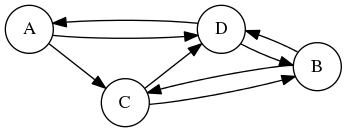
\includegraphics{tex/grafo_H2E6.png}
	\end{center}

Para ver el tiempo medio de retorno a A, podríamos estudiar las  probabilidades, pero es bastante lioso.

Como ya tenemos que es regular sabemos que es irreducible y podemos usar que:

\textit{Tiempo medio de retorno al estado $i$ = inverso de la i-ésima coordenada de la \textbf{distribución límite} = \textbf{única} distribución estacionaria. (es única porque es regular)}

Sabiendo esto calculamos la distribución estacionaria $$\begin{cases}
(\prod)P = (\prod)\\
(\prod) = (x,y,z,t)\\
\end{cases} \rightarrow \begin{cases}
\frac{t}{2} = x\\
\frac{z+t}{2} = y\\
\frac{x+y}{2} = z\\
\frac{x+y+z}{2} = t\\
x + y + z + t=1\\
\end{cases}$$

Y resolviendo este sistema queda que:
$$(\prod) = (x,y,z,t) = \left(\frac{1}{6}, \frac{5}{18}, \frac{2}{9}, \frac{1}{3}\right)$$

Por lo tanto el tiempo medio del primer retorno a A es : \textbf{6}.

Y fijándonos también en la distribución límite vemos que la página más "importante" es \textbf{D}, luego \textbf{B}, \textbf{C} y finalmente \textbf{A}.


% 	Vamos a ver las probabilidades que tenemos de %volver a $A$ para cada número de pasos $n$:
%	\[P_n(\text{ vuelta a A}) = \left\{ %\begin{array}{lcc}
 %            0 &   si  &  n=1\\
  %           \\ 1/4 &   si  &  n=2 \\
   %          \\ 1/8 &   si  &  n=3 \\
    %         \\ 2/16 &   si  &  n=4 \\
     %        \\ 2/32 &   si  &  n=5 \\
      %       \\ 4/64 &   si  &  n=6 \\
       %      \end{array}
   %\right.\]
  % En definitiva estamos teniendo
   %\[P_n = P\left(C \to D \text{ en } n-2 \text{ %pasos}\right) + P\left(D \to D= \text{ en } n-2 %\text{ pasos}\right)\]
   %Vamos a analizar esta probabilidades por separado

   %TO BE CONTINUED (creo que se lo que tiene que %salir, pero no veo clara la explicación %matemática)
   %\begin{itemize}
   %\item
   %\[P_n = P\left(C \to D \text{ en } n-2 \text{ %pasos}\right) \]

   %\item
   %\[ P\left(D \to D= \text{ en } n-2 \text{ %pasos}\right)\]
   %\end{itemize}
\end{problem}

\begin{problem}[7]
	Recuerda que el algoritmo \textit{page rank} sustituye la matriz de transición $P$ por $P_i = (1-ε)P+εE$ donde $E$ es la matríz $N\times N$ con todos sus elementos $1/N$. Explica por qué $P_i$ es una matriz de transición lícita de una cadena de Markov regular cuando $0 \leq t \leq 1$.
	\solution
	\textcolor{blue}{Hecho por Pedro. No fiarse al 100\%}

	Para empezar es evidente que, en caso de corresponderse con una cadena de Markov, $P_ε$ representaría una cadena de Markov regular, pues ella misma tiene todos sus elementos no nulos (tendríasmo $k=1$).

	Puesto que todas las filas de $P$ suman 1, tendremos que las filas de $P_i$ sumarán $1-ε+ε=1$, ya que los elementos de la matríz $E$ también suman 1.

\end{problem}

\begin{problem}[8]
	Consideramos tres páginas web A,B y C. Las dos últimas están enlazadas entre ellas y A enlaza a B. Comprueba que la distribución límite cuando se aplica el algoritmo \textit{page rank} viene dada por
	\[\left(\frac{ε}{3}, \frac{1-2ε/3}{2-ε}, \frac{1-ε+ε^2/3}{2-ε}\right)\]
	Halla autovalores de $P_i$ y con ellos trata de explicar cómo varía la ``velocidad'' de convergencia en términos de ε. Por ejemplo, ¿e bueno o malo coger el número de iteraciones como el inverso de ε?
	\solution

	La matriz de transición de este sistema, suponiendo que todos los enlaces tienen igual probabilidad de ser pulsados, es:
	\[P= \left( \begin{matrix}
	0&1&0\\
	0&0&1\\
	0&1&0\\
	\end{matrix}\right)\]

	La matríz $P_i$ empleada por el algoritmo de \textit{page rank} será de la forma
	$$P_{\epsilon} = (1-\epsilon) \cdot P + \epsilon \frac{1}{3} \left(
	\begin{matrix}
	1&1&1\\
	1&1&1\\
	1&1&1\\
	\end{matrix} \right)$$

	\[P_ε= \left( \begin{matrix}
	ε/3&1-2ε/3&ε/3\\
	ε/3&ε/3&1-2ε/3\\
	ε/3&1-2ε/3&ε/3\\
	\end{matrix}\right)\]

	Puesto que $P_ε$ tiene todos sus elementos no nulos, se trata de una cadena regular y por tanto su distribución límite coincide con la distribución estacionaria. Planteando las ecuaciones habituales para el cáculo de la distribución estacionaria obtenemos exactamente la distribución dada en el enunciado.

	Es decir, bastaría con resolver el sistema
	\[\vx P_ε=\vx\]


	En vez de hacer ese cálculo tal cual lo mejor es hacerlo por trozos.

	$$(\prod) P_{\epsilon} = \left(1-\epsilon\right)\left(\prod\right)P + \frac{\epsilon}{3} \left(\prod\right) \left(
	\begin{matrix}
	1&1&1\\
	1&1&1\\
	1&1&1\\
	\end{matrix} \right) = \left(\prod\right) $$

	Entonces:

	$$ (1-\epsilon)(0,x+z,y) + \frac{\epsilon}{3} (x + y + z) (1,1,1) = (x,y,z) $$

	Si a esta ecuación le añadimos que $ x + y + z = 1$ obtenemos el sistema:

	$$(1-\epsilon)(0,x+z,y) + \frac{\epsilon}{3} (1,1,1) = (x,y,z) \rightarrow \begin{cases}
	\frac{\epsilon}{3}= x\\
	(1-\epsilon)(x+z) + \frac{\epsilon}{3}=y\\
	(1-\epsilon) y + \frac{\epsilon}{3} = z\\
	x + y +z = 1
	\end{cases}$$

	y el resultado es:
	$$(x,y,z) = \left(\frac{ε}{3}, \frac{1-2ε/3}{2-ε}, \frac{1-ε+ε^2/3}{2-ε}\right)$$

	Para la parte de los \textbf{autovalores}:
	Podemos ver que los autovalores de esta matriz son $1,0,ε-1$ y sus autovectores:
	\[(1,1,1) \ \ \left( 1-\frac{3}{ε},1,1\right) \ \ \left(1,-\frac{-3+ε}{-3+2ε},1 \right)\]

	A la hora de estudiar la velocidad de convergencia, tenemos que el tiempo que tardará la matriz diagonal formada por los autovalores en estabilizarse cuando estamos calculando potencias.

	En este caso tenemos dos autovalores constantes e idempotentes por lo que todo depende del último autovalor: $ε-1$. Por tratarse de un número negativo (ε < 1) va a oscilar en torno al 0. Cuanto mayor sea ε más se acercará al 0 y las oscilaciones serán cada vez menores, por lo que convergerá más rápido.
\end{problem}

\begin{problem}[9]
	En una urna hay dos bolas blancas y otras dos negras. Escogemos dos al azar y las pasamos a otra urna. En cada instante se escoge al azar una bola de cada urna y se intercambian.

	Considerando los estados dados por el número de bolas negras en la primera urna más uno, escribe la matriz de probabilidades de transición y halla la distribución límite, probando que existe

	\solution

	Tenemos la matriz:
	\[P= \begin{pmatrix}
	0&1&0\\
	1/4&1/2&1/4\\
	0&1&0
	\end{pmatrix}\]
	La matriz indica que si no tenemos ninguna bola negra en la primera urna, la probabilidad de hacer el movimiento indicado y seguir sin bolas negras en esa urna es 0 ($p_{11}$). Si tenemos una bola negra, la probabilidad de seguir teniendo una bola negra es $p_{22}=1/2$ ya que podemos coger las dos blancas o las dos negras e intercambiarlas (dos de 4 opciones)

	Podemos ver a simple vista que el cuadrado de esa matríz tendrá todos sus elementos no nulos, por lo que la cadena de Markov que estamos trabajando es regular y por tanto existe distribución límite, que coincide con la distribución estacionaria.

	Procedamos pues a calcular esta distribución estacionaria, resolviendo el sistema $(x,y,z) P = (x,y,z)$:

	\[
	(x,y,z) \begin{pmatrix}
	0&1&0\\
	1/4&1/2&1/4\\
	0&1&0
	\end{pmatrix} = (x,y,z)
	\]

	Que nos da el siguiente sistema de ecuaciones:

	\[\begin{cases}
		 \frac{1}{4}y=x\\
		 x+\frac{1}{2}y+z=y\\
		 \frac{1}{4}y=z\\
		 x+y+z=1
	\end{cases} \implies x=z=\frac{1}{6}, y = \frac{2}{3}\]
\end{problem}

\begin{problem}[10]
Suponemos que variamos el esquema del ejercicio anterior considerando las 4 bolas negras y numeradas. En cada paso elegimos un número al azar y cambiamos de urna la bola correspondiente (sin reemplazarla). Halla la distribución estacionaria.
	\solution

	Aunque el enunciado dice que son numeradas, no lo hemos tenido en cuenta en clase, para no complicarlo demasiado.

	En esta ocasión, el estado $i$ representará la situación en que hay $i$ bolas en la primera caja (el elemento de la matriz $p_{02}$ representará la probabilidad de pasar de no tener ninguna bola a tener 2). Con esta consideración, la matriz de transición queda:

	\[P= \left( \begin{matrix}
	0&1&0&0&0\\
	1/4&0&3/4&0&0\\
	0&1/2&0&1/2&0\\
	0&0&3/4&0&1/4\\
	0&0&0&1&0\\
	\end{matrix}\right)\]

	Para buscar la solución estacionaria sólo tenemos que plantear el sistema de ecuaciones habitual:
	\[\vx P = \vx\]

	que, descompuesto en coordenadas, nos queda:

	\[\begin{cases}
		 a=\frac{1}{4}b\\
		 b= a+\frac{1}{2}c\\
		 c= \frac{3}{4} \left(b+d\right)\\
		 d= \frac{1}{2}c+e\\
		 e= \frac{1}{4}d\\
		 a+b+c+d+e=1
	\end{cases} \implies ... \implies (a,b,c,d,e) = \frac{1}{16} (1,4,6,4,1)\]


\end{problem}

\begin{problem}[11]
 Se lanza una moneda hasta que salga una de las secuencias XCC, CXC, CCX. ¿Por
cuál de ellas apostarías?

 Trata de formular el problema como una cadena de Markov (no irreducible) con estados $\{$XX, XC, CX, CC, XCC, CXC, CCX $\}$, donde los estados representan
las dos últimas tiradas o el fin del juego. Calcula el número de tiradas esperado del juego.
	\solution
	\textcolor{blue}{Hecho por Pedro. No fiarse al 100\%}

	La primera pregunta es fácil, lo óptimo sería apostar a la que no apuesten \textbf{Solar} ni \textbf{Cazakas}.

	La cadena de Markov de este ejercicio, con los estados indicados en el enunciado, sería:
	\begin{center}
	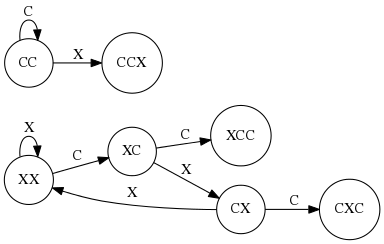
\includegraphics{tex/grafo_H2E11.png}
	\end{center}

	Tal y como nos adelantaba el enunciado, la cadena obtenida no es irreducible. No podemos ir de cualquier estado a cualquier otro en un número finito de pasos.

	TO BE CONTINUED...

	\textcolor{blue}{No se como formular lo que viene ahora correctamente.}

\end{problem}

\begin{problem}[12]
	Da un ejemplo de una cadena de Markov finita regular tal que $P^6$ temga algún ememento nulo, donde $P$ es la matriz de transición.
	\solution
	\textcolor{blue}{Hecho por Pedro. No fiarse al 100\%}

	Basta con escribir un ejemplo tan absurdo como una cadena lineal en la que $p_{ij}=1 \iff i+1=j$ y $P_{ij}=0$ en otro caso.

	Una cadena de este tipo, siempre que sea finita, será regular así que basta con hacerla con más de 6 nodos, de forma que no se pueda llegar del primer estado al último en 6 pasos, lo que provocaría un 0 en la matriz $P^6$.
\end{problem}

\begin{problem}[13]
	Consideramos la cadena de Markov finita con estados en $\ent$, consistente en que en $\ent^+$ damos un paso a la derecha con probabilidad 0.4 y a la izquierda con probabilidad 0.6, mientras que en $\ent^-$ estas probabilidades están intercambiadas. Además, desde el 0 se alcanzan el 1 y el -1 con probabilidad 1/2.

	Como el origen ``atrae'' a los otros estados, se puede probar que el tiempo medio de retorno es finito y la teoría asegura que existe una distribución estacionaria. ¿Cuál es? Por la simetría se puede suponer que toma los mismo valores en los negativos que en los positivos

	\solution
	\textcolor{blue}{Hecho por Pedro. No fiarse al 100\%}

	Aunque la idea sería la de siempre, en este caso el sistema de ecuaciones nos queda con infinitas ecuaciones.

	Vamos a restringirnos a los 2 primeros enteros positivos y negativos y el 0 y supondremos que para los que siguen la distribución será la misma que para los enteros 2 y 3.

	Para representarlo en forma de matriz, consideramos que en los extremenos tenemos tantas posibilidades de quedarnos fijos como posiblidades habría de llegar a esos valores desde estados que quedan excluídos de nuestra simplifiación menos las probabilidades que había de salir de nuestra simplifiación.

	Podemos suponer, sin demasiado riesgo de equivocarnos, que en la distribución estacionaria tendremos los mismos valores en todos los enteros con valor absoluto mayor o igual que 2.

	Por tanto, siendo $a,b,c,d,e$ los valores de los estados $-2,-1,0,1,2$ respectivamente, simulando un movimiento y forzando la estacionalidad de esa solución, tendremos:
	\[\begin{cases}
		a = 0.6a+0.4b\\
		b = 0.6a+0.5c\\
		c = 0.6b+0.6d\\
		d = 0.5c+0.6e\\
		e = 0.4d+0.6e\\
	\end{cases} \implies \begin{cases}
		a = b \\
		0.4 b =0.5c \\
		c = 0.6b+0.6d\\
		0.4d = 0.5c \\
		e = d
	\end{cases} \implies a=b=c=d \ c = 1.2a\]

	De modo que habría infinitas distribuciones estacionarias, que serían todas aquellas que cumplen esa relación:
	\[\left(a,a,1.2a,a,a\right)\]

\end{problem}

\begin{problem}[14]
	El número total de partículas se conserva a lo largo del tiempo en el modelo discretizado de movimiento browniano (paseo aleatorio) en una dimensión. Traduce esto en alguna ley de conservación para le ecuación del calor en $\real$ (con dato de decaimiento rápido) y demuéstrala
	\solution

	\textcolor{blue}{Hecho por Pedro. No fiarse al 100\%}

	El movimiento browniando en una dimensión se corresponde con el análisis del sistema:

	\begin{center}
	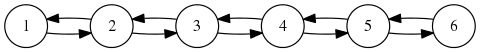
\includegraphics{tex/browniano_1_dim.png}
	\end{center}
	imaginando que se extendiera hasta el infinito por los laterales.

	Consideramos que la probabilidad de coger cualquiera de los dos caminos que parten de un grafo es la misma, de modo que
	\[\prob{X_{n+1}=j}=\frac{1}{2}\prob{X_n = j-1}+\frac{1}{2}\prob{X_n=j+1}\]

	Establezcamos que los valores de tiempo son 0, 1h, 2h, ... y que una partícula se mueve saltando entre los puntos de $ε\ent$ (representados por los nodos de nuestro grafo). Consideramos $S=\ent$ y $X_n$ será la variable aleatoria que toma el valor $j$ cuando la partícula está en la posición $εj$ en tiempo $hn$.

	Como vimos en clase, el análisis combinatorio bien conocido del \textit{paseo aleatorio} unidimensional muestra que, con esta notación, en tiempo $hn=1$ la partícula se aleja del origen del orden de $ε\sqrt{n}$.

	Puesto que queremos que en $hn=1$ la distancia se mantenga acotada, deberámos tomar $h=ε^2/2$\footnote{Consiguiendo que la distancia al origen sea $ε\sqrt{n}=ε\sqrt{\frac{2}{ε^2}} = \sqrt{2}$, que es constante}. Nuestro objetivo será estudiar qué ocurre cuando $ε \to 0$.

	Una vez aclarado esto podemos escribir:
	\[\frac{\prob{X_{n+1}=j}-\prob{X_n=j}}{h}=\frac{\prob{X_n=j-1}+\prob{X_n=j+1}-2\prob{X_n=j}}{ε^2}\]

	Puede comprobarse que la igualdad es cierta de forma sencilla basándose en la relación: $1/2=hε^2$.

	Esperamos que cuando $ε\to 0$, $\prob{X_n=j}$ pueda expresarse como una función buena, que dependa del espacio y el tiempo, $u(x,t)$ con $x=jε$ y $t=hn$. De esta forma la ecuación anterior conduce a:
	\[\frac{u(x,t+h)-u(x,t)}{h}=\frac{u(x-ε,t)+u(x+ε,t)-2u(x,t)}{ε^2}\]
	y podemos observar de manera trivial que esta ecuacuión se corresponde con:
	\[\frac{\partial u}{\partial t}=\frac{\partial^2u}{\partial x^2} \ x \in \real, \ t > 0\]

	Y esta última ecuación no es otra que la \textbf{ecuación del calor}

\end{problem}

\begin{problem}[15]
	Paseamos por $\ent^2$ partiendo del origen y avanzando de uno en uno en una dirección: N, S, E, O, elegida al azar. Demuestra que el número de retornos al origen en a lo más 2M pasos es en media:
	\[\sum_{n=1}^M 4^{-2n}\sum_{k+l=n}(2n)!/(k!)^2(l!)^2\]
	Comprueba que esta serie diverge cuando $M \to \infty$, expresando la suma interior como
	\[4^{n-1}π^{-2}\int_{-π}^π\int_{-π}^π\left(\sin(x)+\sin(y)\right)^{2n}dxdy\]
	\solution


\end{problem}

\section{Hoja 3}
\begin{problem}[1]
Consideramos la función $\appl{f}{\ent_4}{\cplex}$ definida por $10=10$, $f(\pm 1) = -2 \mp 2i$ y $f(2)=-2$. Calcula su desarrollo de Fourier discreto.

\solution

Recordemos que el desarrollo discreto de Fourier se hacía siguiendo la fórmula:
\[f(n)=\frac{1}{N}\sum_m \hat{f}(m)\cdot e \left(\frac{nm}{N} \right) \text{ con } \hat{f}(n)=\sum_m f(m) \cdot e\left(\frac{-nm}{N}\right)\]

En nuestro caso tenemos $N=4$ con $m=0, \pm 1$ y $ 2$. Empezamos calculando los coeficientes de Fourier:

\[\left\{
\begin{array}{rcl}
\hat{f}(0) & =  & e(0) \cdot \left( f(0)+f(1)+f(-1)+f(2) \right)\\
\hat{f}(1) & =  & f(0) \cdot e(0)+f(1) \cdot e \left(-\frac{1}{4}\right) + f(-1)\cdot e \left(\frac{1}{4}\right)+f(2) \cdot e \left(-\frac{1}{2}\right)\\
\hat{f}(-1) & =  &  f(0) \cdot e(0)+f(1) \cdot e \left(\frac{1}{4}\right) + f(-1)\cdot e \left(-\frac{1}{4}\right)+f(2) \cdot e \left(\frac{1}{2}\right)\\
\hat{f}(2) & =  &  f(0) \cdot e(0)+f(1) \cdot e \left(\frac{1}{2}\right) + f(-1)\cdot e \left(-\frac{1}{2}\right)+f(2) \cdot e \left(1\right)
\end{array} \right. \implies \]

\[\implies \left\{
\begin{array}{rcl}
\hat{f}(0) & =  & \left( 10+(-2-2i)+(-2+2i)-2 \right)\\
\hat{f}(1) & =  & 10 +(-2-2i) \cdot (-i) + (-2+2i)\cdot i-2 \cdot (-1)\\
\hat{f}(-1) & =  &  10 +(-2-2i) \cdot i + (-2+2i)\cdot (-i)-2 \cdot (-1)\\
\hat{f}(2) & =  &  10 +(-2-2i) \cdot (-1) + (-2+2i)\cdot (-1)-2 \cdot (1)
\end{array} \right. \implies
\]
\[\implies \left\{
\begin{array}{rcl}
\hat{f}(0) & = 4 \\
\hat{f}(1) & = 8 \\
\hat{f}(-1) & = 16 \\
\hat{f}(2) & = 12
\end{array} \right. \]

Una vez tenemos estos coeficientes calculamos el desarrollo discreto de Fourier:
\[f(n) = \frac{1}{4}\left( 4 + 8 \cdot e \left(\frac{n}{4}\right)+16\cdot e \left(-\frac{n}{4}\right)+12\cdot e \left(\frac{n}{2}\right)\right)\]
\end{problem}

\begin{problem}[2]
	Prueba que la convolución de dos funciones es una operación conmutativa.
	\solution

	Vamos a realizar la prueba considerando funciones $\appl{f,g}{\real}{\cplex}$. En el caso de funciones discretas o 1-periódicas la prueba sería similar.

	Para ver que se trata de una operación conmutativa debemos comprobar que:
	$$f * g = g * f$$

	La definición de convolución nos permite escribir:
	\[(f * g) (x) = \int_{-\infty}^{\infty} f(x - t) g(t) dt \]

	Pero mediante el cambio de variables lineal $u = x - t$, tenemos:
	\[\int_{-\infty}^{\infty} f(x - t) g(t) dt =\int^{\infty}_{-\infty} f(u) g(x - u) du \]

	Y aplicando nuevamente la definición de convolución llegamos a
	\[\int^{\infty}_{-\infty} f(u) g(x - u) du = (g * f)(x) \]

	Con lo que queda probado
	\[(f * g) (x)  = (g * f) (x) \]


\end{problem}

\begin{problem}[3]

	Consideramos las funciones 1-periódicas reales que en [0,1] coinciden, respectivamente con $\min(x,1-x)$ y con $(-1)^{[2x]}$ donde $[\cdot ]$ indica la parte entera. Calcula sus coeficientes de Fourier. Expresar la primera serie de Fourier en términos de cosenos y la segunda en términos de senos.
	\solution

%	\yoP

	La primera función parte del origen y asciende como $y=x$ hasta llegar a $x=y=0.5$ y posteriormente desciende de forma lineal hasta llegar a $x=1, y=0$.


	Vamos a calcular su desarrollo de Fourier, puesto que en esta ocasión tenemos $\appl{f}{\mathbb{T}}{\cplex}$ la fórmula que debemos aplicar es:

	\[f(x)=\sum_{n=-\infty}^{\infty} \hat{f}(n)e(nx) \text{ donde } \hat{f}(n)=\int_0^1 f(x)e(-nx)\]

	Calculamos pues los coeficientes de fourier, que quedan de la forma:
	\[\hat{f}(n)=\int_0^{1/2} x e^{-2πnxi}dx+\int_{1/2}^1 \left(\frac{1}{2}-x\right)e^{-2πnxi}dx= \]
	\[=\left. -\frac{e^{-2πinx}(2πinx+1)}{(2πin)^2}\right|_0^{1/2} + \left. \left(- \frac{e^{-2πinx}}{4πin}+\frac{e^{-2πinx}(2πinx+1)}{(2πin)^2}\right) \right|_{1/2}^1 = \]
	\[=...=\frac{-e^{-πin}(πin+1)-1}{4π^2n^2}-\frac{e^{-2πin}-e^{-πin}}{4πin}+\frac{e^{-2πin}(2πin+1)-e^{πin}(πin+1)}{4π^2n^2}=\]
	\[=\frac{-e^{-πin}(πin+1)-1-e^{-2πin}(πin)+e^{-πin}(πin)+e^{-2πin}(2πin+1)-e^{πin}(πin+1)}{4π^2n^2}=\]
	\[=\frac{-e^{πin}(πin)-2e^{-πin}+e^{-2πin}-1}{4π^2n^2}=\frac{(-1)^{n+1}(πin)+2(-1)^{n+1}}{4π^2n^2}\]

	\textcolor{blue}{Como no estoy nada seguro de estas cuentas no voy a seguir avanzando. Lo que habría que hacer a continuación es escribir el desarrollo de fourier sustituyendo $\hat{f}$ por la última fracción calculada y basarnos en las ecuaciones de Euler para pasar de complejos a funciones que sólo contengan cosenos.}

	La segunda función oscila entre $-1$ y $1$ y podemos verla claramente representada en la siguiente gráfica.
	\begin{center}
		\inputtikz{fourier/onda_cuadrada}
	\end{center}

	Calculamos ahora los coeficientes de Fourier, con lo que tenemos:

	$$ \hat{f}(n) = \int^{1}_{0} f(x) e(-nx)dx = \int^{1/2}_{0} e(-nx)dx - \int^{1}_{1/2} e(-nx) dx =  \left.\frac{-1}{2 \pi i n} e(-nx) \right|^{1/2}_{0} +\left. \frac{1}{2 \pi i n} e(-nx)  \right|^{1}_{1/2} $$

	$$ = \frac{-1}{2 \pi i n}\left( e\left( -\frac{n}{2} \right) -1 \right) + \frac{1}{2 \pi i n}\left(1 - e\left( -\frac{n}{2} \right) \right)$$

	Como $e(-1/2) = e^{2 \pi i (-1/2)} = -1$ nos queda:

	$$ \hat{f}(n) = \frac{1}{\pi i n} (1 - e(-n/2)) = \begin{cases}
	0 & \mbox{ si } n\text{ par} \\
	\frac{2}{\pi i n} & \mbox{ si } n \text{ impar}
	\end{cases} $$


	$$ f(x) = \frac{2}{\pi i} \sum\limits^{\infty}_{n = -\infty \text{ y } 2 \nmid n} \frac{e(nx)}{n} $$

	Teniendo en cuenta que
	\[e(nx) = \cos(2 	\pi n x) + i \sin(2 \pi n x)\text{ y }\frac{e(nx)}{n} + \frac{e(-nx)}{-n} = 2i \frac{\sin(2\pi n x)}{n}\]

	Nos queda:

	$$ f(x)= \frac{2}{\pi i} \sum\limits^{\infty}_{n = 1\text{ y } 2 \nmid n}  2i\frac{\sin (2 \pi n x)}{n} = \frac{4}{\pi} \sum^{\infty}_{k=0} \frac{\sin(2 \pi (2 k + 1) x)}{2k + 1} $$

\end{problem}

\begin{problem}[4]
	Calcula la transformada de Fourier de la función característica $f$ de un intervalo [-a/2,a/2]$\subset \real$. Estudia qué ocurre con $a^{-1}f$ y $a^{-1}\hat{f}$ cuando $a \to 0$. Teniendo esto en cuenta, ¿cómo parece que habría que definir $\int_{-\infty}^{\infty}e(\xi x)d\xi $? Esta fórmula se emplea con mucha frecuencia en Física sin más explicaciones.

	\solution
	Es sencillo ver que
	\[\lim_{a \rightarrow 0} a^{-1} f(x) = \lim_{a \rightarrow 0} a^{-1} \chi_{[-a/2,a/2]} (x) = 0\ \forall x\neq 0\]

	puesto que si $x \neq 0$, en algún momento tendremos $|a/2| < |x|$ de modo que la $x$ estará fuera del conjunto sobre el que $f$ es función característica y por tanto tendremos $ \lim_{a \rightarrow 0} a^{-1} \cdot 0 = 0$

	Por otro lado
	\[x = 0 \implies \lim_{a \rightarrow 0} a^{-1} f(x) = \lim_{a \rightarrow 0} a^{-1} = \infty \]
	puesto que todos los intervalos $[-a/2,a/2]$ contienen el 0 de modo que $f(x)=1$ siempre.

	Podemos ver también que:
	$$\int^{\infty}_{-\infty} a^{-1} f(x) = 1 $$

	Por lo que, en cierto modo, $a^{-1} \convs[][a][0]$ delta de Dirac.

	Vamos a estudiar ahora el comportamiento de $a^{-1}\hat{f}$:

	$$\lim_{a \rightarrow 0} a^{-1} \hat{f}(\xi) = \lim_{a \rightarrow 0} a^{-1} \int^{\infty}_{-\infty} f(x) e(-x \xi) dx = \lim_{a \rightarrow 0} a^{-1} \int^{a/2}_{-a/2} e(-x\pi) dx = \lim_{a \rightarrow 0} a^{-1} \cdot 2 \cdot \frac{\sin (2 \pi \xi a/2)}{2 \pi \xi} =1 $$

	Esto sugiere que $\hat{\delta} = 1$

	Aplicando ahora la fórmula de inversión  tenemos
	\[\delta (x) = \int\limits^{\infty}_{-\infty} 1 \cdot e(x \xi) d \xi\]

	con lo que parece que hemos alcanzado una definición posible para la integral pedida.

	\obs Como podemos observar, la integral no converge. Vale $0$ en todo punto salvo en 1, que es $\infty$.

\end{problem}

\begin{problem}[5]
Para trata de forma discreta ondas muy oscilatorias hay que tomar muestras muy grandes para limitar ambigüedades graves. Sea una señal $f(x)=Ae(vx)+Be(-vx)$ con $v \in \real^+$. Supongamos que al extraer $N$ muestras se obtiene $f(j/N)=0$ para $0 \leq j < N$, es decir, lo mismo que se obtendría muestreando la función nula. ¿Cuáles son los posibles valores de $v$?. Explica por qué esto sugiere que el número de muestras debe ser al menos el doble de la frecuencia de una señal (la generalización de esto es el \textit{Teorema de Nyquist})
\solution

Tenemos una señal de la forma
\[f(x)=Ae(vx)+Be(-vx)\]

Puesto que tenemos que $f(j/N)=0$ para todo $j$, nos queda:
\[Ae\left(\frac{vj}{N}\right)+Be\left(-\frac{vj}{N}\right)=0 \implies e\left(2\frac{vj}{N}\right)=-\frac{B}{A}\]
y, como en particular esto es cierto para $j=0$ tenemos que $B=-A$.

Puesto que $B$ y $A$ son constantes, tenemos que para calcular valor de $j$, $e\left(2\frac{vj}{N}\right)$ debe valer siempre lo mismo. La única forma de que esto ocurra necesitamos que
\[\frac{2v}{N}\in \ent\]
ya que así, al descomponer la función $e$ como combinación de senos y cosenos, tendremos coseno y seno de múltiplos enteros de $2π$, que nos garantiza la constancia en su valor.

Por tanto, nos queda la igualdad $2v=NK$ siendo $K$ un entero positivo. Para evitar que esto pueda producirse basta con tomar $N>2v$.
\end{problem}

\begin{problem}[6]
Si en una imagen en formato JPEG hacemos cero todos los coeficientes de Fourier excepto los $a_{00}$ que corresponden a la función $\phi_{00}$, ¿qué ocurrirá?
\solution

La imagen se verá totalmente pixelada, pues para cada bloque de $8\times 8$ estaremos tomando el color que tenía el pixel $(0,0)$ del bloque.

\end{problem}

\begin{problem}[7]
Halla los coeficientes antes de cuantificar una imagen JPEG que consta sólo de los píxeles de la primera columna en blanco (valor=255) y el resto negros (valor=0), tratando de expresarlos de manera lo más simple posible
\solution

\yoP

\textcolor{green}{corregido en clase}

Podemos estudiar el desarrollo de Fourier de la función que nos da el color para cada uno de los tres colores básicos RGB que, en este ejemplo, serán los tres iguales.

Los resultados experimentales vistos en clase muestran que el resultado será una función real, es decir, que sólo dependerá de cosenos.

Aplicamos pues la transformada coseno discreta:
\[F=\sum_{n=0}^7\sum_{m=0}^7 a_{nm}\phi_{nm} \text{ con } \phi_{nm}(l,k)=\cos\left(\frac{πn}{16}(2k+1) \right) \cos\left( \frac{πm}{16}(2l+1)\right)\]

Despejando podemos ver que los coeficientes se calculan según la siguiente fórmula, que aparece en los apuntes del profesor:
\[a_{nm}=\frac{α_nα_m}{64}\sum_{k=0}^7\sum_{l=0}^7F(k,l) \phi_{nm}(l,k) \text{ donde } α_n=2 \text{ si } n\neq0 \text{ y }1 \text{ si }  n = 0 \]

Todos los bloques que no estén en la frontera izquierda de la imagen tendrán todos sus coeficientes nulos puesto que al calcular $a_{nm}$ tendremos $F=0$.

Por tanto, el caso interesante lo constituyen los cuadrados fronterizos. Puesto que $F(k,l)=0 \forall l\neq 0$ podemos escribir:
\[a_{nm} = \frac{α_nα_m}{64}\sum_{k=0}^7F(k,0)\phi_{nm}(0,k)=\frac{α_nα_m}{64}\sum_{k=0}^7F(k,0)\cos\left(\frac{πn}{16}(2k+1) \right) \cos\left( \frac{πm}{16}\right)\]

Sabemos que todos los píxeles de la frontera tienen el mismo color, 255, de modo que $F(k,l)=255$ por lo que podemos simplicar la fórmula y escribir:
\[a_{nm}=\frac{α_nα_m}{64}\cdot 255 \cdot \sum_{k=0}^7\cos\left(\frac{πn}{16}(2k+1) \right) \cos\left( \frac{πm}{16}\right)\]

Vemos que
\[\sum_{k=0}^7\cos\left(\frac{πn}{16}(2k+1) \right) = \begin{cases}
8 \textbf{ si } n= 0\\
0 \textbf{ si } n\neq0
\end{cases}\]

Entonces como la parte real del sumatorio de exponencial da el sumatorio de cosenos puedo calcular:
\[ \sum_{k=0}^7e\left(\frac{n}{32}(2k+1) \right)\]
que es una progresión geométrica.

Y luego cojo su parte real

\textcolor{blue}{Yo ya lo veo bastante simple}

\end{problem}

\begin{problem}[8]
Una imagen JPEG que consta de una línea horizontal negra gruesa de lado a lado
en un fondo blanco no es invariante por traslaciones; es decir, el tamaño del fichero depende de la altura a la que está la línea. Explica este fenómeno. ¿Para qué grosores y posiciones habrá mayor compresión?

\solution

\yoP

\textcolor{green}{corregido en clase}


El tamaño depende de la altura de la linea, vamos a ver porqué.

En JPEG se dividian los bloques en 8 y se interpretaba cada bloque por Fourier.

Pensemos primero en los casos de linea con grosor 8.

En la situación de que la linea esté justo en el centro de los bloques la función que analizamos Fourier en cada bloque es constante. Es decir $a_{00} = algo$ y e resto nulos.

Si no cuadra con el bloque, por ejemplo cogemos un pixel de los bloques de arriba, vemos que en los 6 bloques restantes la función no es constante por lo tanto hay $a_{ij} \neq 0$ y $a_{00}\neq 0$ por lo tanto ocupa más.

Esto es porque en todos los cuadrados que contienen la linea , hay un cambio abrupto de blanco a negro en solo un pixel.

Para entender porqué es esto recordamos que JPEG expresaba cada cuadrado como combinación lineal de los cuadrados "base".
$$f(k,l) = \sum_{n,m = 0}^{7} a_{nm} \varphi(k,l)$$



%Si nos fijamos en el ejercicio anterior, vimos que todos los cuadrados que no tocaran la línea tendrían todos sus coeficientes iguales. En el ejercicio anterior eran 0 y en este caso 255 (suponemos fondo blanco).

%En cualquier caso, esta extensa repetición de caracteres facilita la compresión del fichero.

%Por tanto la mayor compresión se alcanzará cuando la línea se situe en uno de los extremos de la imagen (superior o inferior) ya que será cuando menos cuadrados $8\times 8$ interesequen con ella.

\end{problem}

\begin{problem}[9]
Demuestra que los polinomios de Chebyshev $T_n(x)=\cos(n \arccos x)$ son realmente polinomios para $x \in [-1,1]$ y que satisface
\[T_{n+1}(x)=2xT_n(x)-T_{n-1}(x) \text{ para } n \geq 1\]
\solution

\yoP

Para empezar vamos a comprobar que se satisface la ecuación recursiva.

\[T_{n+1}(x)=\cos((n+1)\arccos x) = \cos(n\arccos x)\cos(\arccos x)-\sin(n \arccos x)\sin(\arccos x) =\]
\[=T_n(x)x-\sin(n \arccos x)\sqrt{1-x^2}\]

Por otro lado tenemos:
\[T_{n-1}(x)=\cos((n-1)\arccos x) = \cos(n\arccos x)\cos(\arccos x)+\sin(n \arccos x)\sin(\arccos x) =\]
\[T_n(x)x+\sin(n \arccos x)\sqrt{1-x^2} \implies \sin(n \arccos x)\sqrt{1-x^2} =T_{n-1}(x)-T_n(x)x\]

Y sustituyendo este resultado en la ecuación anterior obtenemos el resultado buscado.

Una vez hemos probado que la ecuación recursiva es cierta nos basta con fijarnos en que $T_1(x)=\cos(\arccos(x))=x$. Sabiendo además que $T_0(x)=1$ queda perfectamente claro que la ecuación recursiva nos lleva a obtener polinomios.

\textcolor{green}{Otra forma de hacerlo (hecho en clase)}


Llamamos $\arccos x = y$ entonces
$$T_n(x) = \cos (ny)$$

Intentamos relacionar $T_{n+1}(x)$ con $\cos(ny)$. Para ello vemos que:

$$T_{n+1}(x) = \cos((n+1)y) = \cos(ny) cos y - \sen(ny) \sen y$$

Vemos que $\cos(ny) = T_n(x)$ , el $\cos y= x$ y para los senos utilizamos las fórmulas de procudo de cosenos de forma que nos queda que:
$$ \sen(ny) \sen y = \frac{\cos((n+1)y) - \cos((n-1)y)}{2} = \frac{T_{n+1}(x) - T_{n-1}(x)}{2}$$

Teniendo esto ya podemos ver que:
$$\implies T_{n+1}= x\cdot T_n + \frac{T_{n+1} - T_{n-1}}{2} \iff T_{n+1} = 2xT_n - T_{n-1}$$

\end{problem}

\begin{problem}[10]
Prueba que para funciones impares los coeficientes con índice par en el desarrollo de Chebyshev-Fourier son nulos. Busca un análogo para funciones pares.
\solution

\yoP

Recordemos que una función impar es cualquier función que satisface
\[f(-x)=-f(x)\]

El desarrollo de Chebyshev-Fourier de una función $f(x)$ dada es de la forma:
\[f(x)=a_0+2\sum_{n=1}^{\infty}a_nT_n(x) = a_0+2\sum_{n=1}^{\infty}a_n\cos(n \arccos x)\]
Por otro lado, el desarrollo de Chebyshev-Fourier de $f(-x)$ tenemos:
\[f(-x)=a_0+2\sum_{n=1}^{\infty}a_n\cos(n \arccos (-x))=a_0+2\sum_{n=1}^{\infty}a_n\cos(n (π - \arccos x))=\]
\[=a_0+2\sum_{n=1}^{\infty}a_n\left( \cos(nπ)\cos(n\arccos x) + \sin(nπ)\text{algo}\footnote{No nos importa puesto que irá multiplicado por 0}\right) =a_0+2\sum_{n=1}^{\infty}a_n \cos(nπ)\cos(n\arccos x)=\]
\[=a_0+2\sum_{n=1}^{\infty}a_n(-1)^n\cos(n\arccos x)\]

Sabiendo que $f$ es una función impar, igualamos los dos desarrollos obtenidos invirtiendo el signo en el segundo. Así nos quedan dos desarrollos exactamente idénticos en los términos impares pero con signos opuestos en todos los pares. La única opción para que se mantenga la igualdad es que estos términos de índice par sean nulos.

Por otro lado las funciones pares son aquellas que cumplen
\[f(x)=f(-x)\]

En este caso, igualar los desarrollos anteriormente calculados (de $f(x)$ y $f(-x)$) nos quedarían dos series idénticas en los términos pares y con signos opuestos en los impares. La única forma de que ambas series sean idénticas es que esos términos impares sean nulos.

\textcolor{green}{Otra forma de hacerlo (hecho en clase)}

Tenemos que
$$a_n = \int_{0}^{1} f(\cos(2\pi x)) \cos (2\pi nx) dx$$
Esto lo hemos sacado de la fórmula de los coeficientes de Fourier:
$$F(x) = f(\cos(2\pi x)) \rightarrow a_n = \int_{0}^{1} F(x) e(-nx)dx$$

Vemos que \textbf{para f impar} $\implies a_{2k} = 0$

Vamos a probar esto último:

Hacemos un cambio de variable en la integral de forma que $x = t+\frac{1}{2}$

$$a_{2k} = \int_{0}^{1}... = \int_{-\frac{1}{2}}^{\frac{1}{2}} f(\cos(2\pi t + \pi)\cdot \cos(2 \pi 2kt + 2 \pi k)dt $$

Vemos que $\cos(2 \pi 2kt + 2 \pi k) = \cos(2\pi 2k t)$ y que $f(\cos(2\pi t + \pi) = f(-\cos(2\pi t) = -f(\cos(2\pi t)$

Entonces
$$a_{2k} = -\int_{-\frac{1}{2}}^{\frac{1}{2}} f(\cos(2\pi t)\cdot \cos(2 \pi 2kt)dt$$
y por ser 1-periódica nos queda
$$a_{2k} = -\int_{a}^{a+1}  f(\cos(2\pi t)\cdot \cos(2 \pi 2kt)dt$$
y para $a=0$

$$\implies \int_{0}^{1} .... dx = -\int_{0}^{1}.... dt \implies \int_{0}^{1} = 0 \implies a_{2k} = 0$$
\end{problem}

\begin{problem}[11]
Explica cómo calcularía la función tangente para cualquier valor real si tu calculadora sólo te permitiera evaluarla en $[-π/4,π/4]$. Consiera el desarrollo de Chebyshev-Fourier de $f(x)=\tan(πx/4)$ truncando hasta los dos primeros coeficientes no nulos. Con ayuda de un ordenador, aproxima estos dos coeficientes con 6 cifras decimales y comprueba la precisión al proximar $\tan (3/4)$. Compara el resultado obtenido al emplear dos términos no nulos de la siere de Taylor de $f$
\solution

Para empezar sabemos que la función tangente es una función $\pi$-periódica con la siguiente gráfica:

\begin{center}
	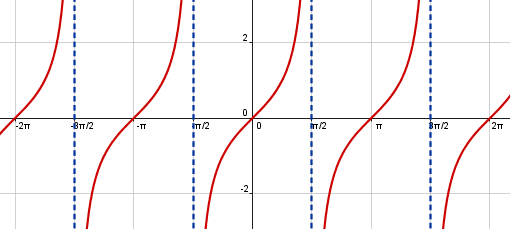
\includegraphics{img/grafica_tangente.png}
\end{center}

Podemos observar que el período no se da en $[-π/4,π/4]$ sino en $[-π/2,π/2]$. No obstante, tenemos que
\[\tan\left(\frac{π}{2}-x\right)=\frac{\sin(π/2-x)}{\cos(π/2-x)}=\frac{\cos(x)}{\sin(x)}=\frac{1}{\tan(x)}\]

Así podemos obtener el valor de la tangente para un punto comprendido entre π/4 y π/2 puesto que al restarle π/2 a un valor de este tipo caemos en la zona conocidoa: $[-π/4,π/4]$

Sabemos que el desarrollo de Chebyshev-Fourier es de la forma:
\[f(x)=a_0+2\sum_{n=1}^{\infty}a_nT_n(x) \text{ con } T_n(x)=\cos(n \arccos(x))\]

Puesto que nuestra función $f$ es impar sabemos que los coeficientes con $n$ par serán nulos

Calculamos $a_1$ y $a_3$:

\[a_1 = \int_{0}^{1} \tan(\frac{\pi}{4} \cos (2\pi x)) \cdot \cos(2 \pi x) dx = 0.469225\]
\[ a_3 = 0.028585\]

Entonces

\[ \tan\frac{3}{4} = f(\frac{\pi}{3})\simeq 2 a_1 T_1(\frac{3}{\pi}) +2 a_3 T_3 (\frac{3}{\pi}) = 0.931506\]



\end{problem}

\begin{problem}[12]
Sabiendo que $\int_{-\infty}^{\infty}e^{-x^2}dx = \sqrt{π}$ calcula la transformada de Fourier de $f(x)=e^{-αx^2}$, α>0, utilizando un cambio de variable $x \to μx+\upsilon, \upsilon \in \cplex$. Justifica que este cambio complejo es lícito
\solution

\yoP

Para calcular esta transformada de Fourier nos apoyaremos en la fórmula:
\[f(x)=\int_{-\infty}^{\infty}\hat{f}(ε)e^{-εx}dε \text{ siendo } \hat{f}(ε)=\int_{-\infty}^{\infty}f(x)e^{-εx}dx\]

Calculamos primero los coeficientes de la serie:
\[\hat{f}(ε)=\int_{-\infty}^{\infty}f(x)e(εx)dx = \int_{-\infty}^{\infty}e^{-αx^2}e(-εx)dx = \int_{-\infty}^{\infty}e^{-αx^2-iεx}dx\]

Atendiendo a la indicación del enunciado, hacemos el cambio de variable $x=μt+\upsilon$, con lo que deberemos cambiar $dx=μdt$ obteniendo:
\[ \int_{-\infty}^{\infty}e^{-αx^2-iεx}dx =  \int_{-\infty}^{\infty}e^{-α(μt+\upsilon)^2-iε(μt+\upsilon)}dx = \int_{-\infty}^{\infty}e^{-αμ^2t^2-α\upsilon^2-2αμ\upsilon t-iεμt-iε\upsilon}dx\]

El cambio de variable que hicimos tenía dos constantes que no hemos especificado y cuyo valor no altera los pasos seguidos hasta llegar a este punto. Si escogemos bien $\upsilon$ podemos eliminar el termino $t$ del exponente.

Para ello necesitamos
\[-2αμ\upsilon =iεμ \implies \upsilon=\frac{iε}{-2α}\]

Además, dada la información que nos proporciona el enunciado, nos interesa que el coeficiente del término $t^2$ sea 1. Para ello basta con tomar $μ=\sqrt{α}$.

Por tanto ya tenemos completamente identificado el cambio de variable que vamos a realizar. Con él, obtenemos:
\[\int_{-\infty}^{\infty}e^{-αμ^2t^2-α\upsilon^2-2αμ\upsilon t-iεμt-iε\upsilon)}dx = \int_{-\infty}^{\infty}e^{-t^2-α\upsilon^2-iε\upsilon}dx = \sqrt{π}\cdot e^{ε^2/(4α)-ε^2/(2α)}\]

\end{problem}

\begin{problem}[13]
El filtro de convolución \textit{sharpen} para imágenes se representa a veces con una matriz $3 \times 3$ cuyos elementos son $-1$, excepto el central que es $9$. Intenta adivinar su efecto visual.
\solution

\end{problem}

\begin{problem}[14]
Explica por qué si se sabe que la densidad es una función radial, entonces basta una proyección para reconstruirla por tomografía. Demuestra que en este caso una fórmula para hacerlo es
\[ρ(x,y)=\int_{\infty}^{\infty} \int_0^π |r|\hat{P}_0(r)e(r\cos(\theta) \sqrt{x^2+y^2})d\theta dr\]
\solution

Tenemos la siguiente fórmula:
\[\rho (x,y) = \int_{0}^{2\pi}\int_{0}^{\infty} r \widehat{P_{\theta}}(r) e(xr\cos\theta + y r \sin\theta) dr d\theta\]
Lo que tenemos que utilizar es que para $\rho$ radial $\implies P_{\theta} = P_0$ (No depende de $\theta$).

Entonces $\widehat{P_{\theta}} = \widehat{P_0}$

$\rho$ radial $\implies \rho(x,y) = \rho(\sqrt{x^2+ y^2}, 0)$

Entonces tenemos que
\[\rho(x,y) = \rho(\sqrt{x^2+ y^2}, 0) = \int_{0}^{2\pi}\int_{0}^{\infty} r \widehat{P_0}(r) e(\sqrt{x^2 + y^2}r\cos\theta) dr d\theta\]

Y ahora , para que nos quede como en el enunciado, podemos hacer dos cosas: La primera es hacer un cambio a un tipo de polares "raras"

La segunda es ver que tengo 
\[\int_{0}^{2\pi}\int_{0}^{\infty} r... = \int_{0}^{\pi}\int_{0}^{\infty} r... + \int_{\pi}^{2\pi}\int_{0}^{\infty} r...\] 

 Para transformar el segudo par de integrales lo que hago es transformar $\theta \rightarrow \theta + \pi$, que puedo hacerlo porque el coseno es periódico,  y $r \rightarrow -r$

El cambio de $\theta$ me cambia los límites de la integral a $\int_{0}^{\pi}$ y el segundo cambio me deja $\int_{-\infty}^{0} -r ....$

Una vez que teneos esto, al hacer la suma ya nos queda $\int_{0}^{\pi} \int_{-\infty}^{\infty} |r|... drd\theta$
\end{problem}

\begin{problem}[15]
Halla $P_{\theta}(t)$ al hacer tomografías de las secciones de:

\ppart Una barra homogénea de denisdad 1 y radio 1
\ppart Esta barra vaciada hasta radio 1/2
\ppart El resultado de rellenar el hueco central con un material de densidad 2
\solution

\ppart $P_{\theta}(t) = \int_{r_{\theta, t}} \rho$

Justo debajo de la línea, donde $t = 0$ $P_{\theta}(0) = 2$

Entonces la solución general sería
\[P_{\theta}(t) \begin{cases}
2 \sqrt{1-t^2} \text{ si } -1<t<1\\
0 \text{ en otro caso}
\end{cases}\]

\ppart Mientras los rayos no atraviesen lass parte vacía, el resutado es igual que el apartado anterior.

Cuando $|t| \qeq 1$  ( osea que no pasa por la barra) es 0, igual que el apartado anterior.

Cuando si atravesamos la parte vacía tenemos el total $2 \sqrt{1-t^2}$ y le tenemos que restar la parte hueca $2 \sqrt{{\frac{1}{2}}^2 - t^2}$

En general nos queda
\[ P_{\theta}(t)= \begin{cases}
2 \sqrt{1-t^2} \text{ si } \frac{1}{2} \leq |t| \leq 1\\
0 \textbf{ si } |t| \geq 1\\
2 \sqrt{1-t^2}- 2 \sqrt{{\frac{1}{2}}^2 - t^2}\text{ si } |t| \leq \frac{1}{2}
\end{cases}\]

\end{problem}

\begin{problem}[16]
Un modelo natural para la temperatura en el interior de la Tierra a profundidad $x$ (pequeña) es que $u(x,t)$ es periódica en $t$ de período un año por efecto de las estaciones, y entonces
\[u(x,t)=\sum c_n(x)e(nt)\]
Deduce $c_n(x)=a_ne^{-x(1\pm i)\sqrt{π|n|}}$ de la ecuación del calor $u_t=u_{xx}$, suponiendo $u(+\infty, t)< \infty$, con $a_n$ los coeficientes de Fourier de la temperatura en la superficie y $\pm$ el signo de $n$.
\solution


\end{problem}

\begin{problem}[17]
Halla $u(x,t)$ en el problema anterior cuando $u(0,t)=λ_0+\sin(2πt)$ (el verano corresponde a t = 1/4 y el inverno a t=3/4). Deduce que las estaciones no actúan con la misma intensidad ni al mismo tiempo en la superficie que en el interior.
\solution

\end{problem}

\begin{problem}[18]
Explica por qué si $\appl{f}{\ent_{2^k}}{\cplex}$ entonces $f_p(n)=f(2n)$ y $f_i(n)=f(2n+1)$ se pueden considerar funciones $\appl{\hat{f}}{\ent_{2^{k-1}}}{\cplex}$ y satisfacen $\hat{f}(n)=\hat{f}_p(n)+e(-n/2^k)\hat{f}_i(n)$. La iteración de esta fórmula da lugar a la importantísima $FFT$. Suponiendo los $e(n/2^k)$ conocidos de antemano, explica por qué esto ahorra operaciones al calcular $\{\hat{f}(n)\}_{n=1}^{2^k}$
\solution

Hacemos el desarrollo de Fourier para $f_p, f_i$: \begin{gather*}
\hat{f}_p(n) = \sum_{m = 0}^{2^{k-1}} f(2m) e\left(\frac{-mn}{2^{k-1}}\right) \\
\hat{f}_i(n) = \sum_{m = 0}^{2^{k-1}} f(2m + 1) e\left(\frac{-mn}{2^{k-1}}\right) \\
\end{gather*}

Vamos a multiplicar $\hat{f}_i(n)$ por $e(-n/2^k)$. Para ello, vemos primero cómo nos quedan las exponenciales: \[ \fe{\frac{-mn}{2^{k-1}}} · \fe{\frac{-n}{2^k}} = \fe{\frac{-2mn - n}{2^k}} = \fe{\frac{-n(2m+1)}{2^k}} \]

Vemos que lo que nos queda es como las exponenciales impares del desarrollo de $\hat{f}(n)$. De hecho, si multiplicamos por dos arriba y abajo en la exponencial de $\hat{f}_p(n)$ \[ \fe{\frac{-mn}{2^{k-1}}} = \fe{\frac{-2mn}{2^k}} \] y entonces, la identidad del enunciado nos queda que \[ \hat{f}_p(n) + \fe{\frac{-n}{2^k}} \hat{f}_i(n) = \sum_{m=0}^{2^{k-1}} \left(f(2m)\fe{\frac{-2mn}{2^k}} + f(2m+1)\fe{\frac{-n(2m+1)}{2^k}} \right) \]

Si nos fijamos, tenemos exactamente todos los términos de $\hat{f}(n)$, así que ya lo tenemos todo listo.
\end{problem}



\newpage
\section{Hoja 4}
\begin{problem}[1]
	Sean $0 \leq p \leq 1$ y $q =1-p$. Comprueba que la entropía de $\{a,b\}$ con $p_1=p$, $p_2=q$ es la mitad que la de $\{A,B,C,D\}$ con $p_1=p^2, \ p_2=p_3=pq, \ p_4=q^2$. ¿Cómo se generaliza este hecho?
	\solution

	La entropía de $\{a,b\}$ se calcula como:
	$$H_1 = -p \log_2 p - q \log_2q$$

	Y la entropía del $\{A,B,C,D\}$ es:
	\begin{gather*}
	H_{2} = -p^2\log_2 p^2 - 2pq(\log_2p + \log_2q) - q^2\log_2 q^2 =\\
	= -2p^2\log_2 p - 2pq\log_2p - 2pq\log_2q - 2q^2\log_2q
	\end{gather*}

	Entonces
	$$H_{S_2}= (-2p^2-2qp)\log_2p + (-2q^2 - 2qp)\log_2q$$

	y como
	$$-2p^2-2qp= -2p(p+q) \eqreason{q=1-p, p+(1-p)=1} -2p$$
	$$-2q^2 - 2qp = -2q(q+p) =-2q$$

	Es fácil ver que $$H_{2} = 2H_1$$

	¿Cómo se generaliza éste hecho?\\
	La generalización de este hecho es que la entropía de una cadena de N símbolos es la entropía multiplicada por N.

	\yoP

	Analizando las probabilidades dadas tenemos que el segundo conjunto representa las diferentes posibilidades al tomar dos elementos de $\{a,b\}$ con sus probabilidades respectivas. Así, los elementos de ese segundo conjunto que nos dan representan:
	\[A= a,a \ B=a,b \ C=b,a \ D=b,b\]

	La generalización de este hecho sería que dado un conjunto con ciertos elementos donde cada elemento tiene una cierta probabilidad de aparición, si tomamos el conjunto formado por las combinaciones posibles de dos elementos, la entropía se duplica.

\end{problem}
 \begin{problem}[2]
 	Tenemos una moneda trucada en la que sale cara sólo el 30\% de las veces. ¿Qué tiene más entropía (cantidad de información), lanzar un dado una vez o lanzar la moneda trucada tres veces?
 	\solution
 	Sea $p$ la probabilidad de sacar cara con esta moneda tenemos:
 	$$p = 0.3$$

 	En un dado la probabilidad de cada número es
 	$$p_i = \frac{1}{6}$$

 	Vamos a calcular la dos entropías que se nos pide:

 	\begin{enumerate}
 		\item \textbf{Tirar una vez el dado}
 		$$H_1 = - \frac{1}{6} \log_2 \frac{1}{6} .... - \frac{1}{6} \log_2 \frac{1}{6} = - \log_2 \frac{1}{6} = \log_2 6 \approx 2.5849 \ \footnote{Recordatorio cambio de base del logaritmo: $\log_b(x) = \frac{\log(x)}{\log(b)}$} $$

 		\item \textbf{Tirar 3 veces la moneda}

 		Se podría calcular $H_2$ hallando las probabilidades de cada una de las 8 probabilidades. Pero vamos a hacerlo de forma más corta:

 		$$H_2 = 3H_{\text{tirando una vez la moneda}}$$

 		Esto se puede hacer porque los sucesos son independientes\footnote{Puede deducirse a partir de la generalización del ejercicio anterior.}.

 		$$H_2 = 3\cdot(-0.3 \log_2 0.3 - 0.7 \log_2 0.7) \approx 2.6438$$
 	\end{enumerate}

 	Podemos comprobar que tenemos una mayor entropía al lanzar la moneda trucada tres veces.
 \end{problem}

\begin{problem}[3]
	Prueba que la entropía de un conjunto con probabilidades $p_i$ cumple
	\[H \leq -\sum p_i \log(q_i)\]
	cualesquiera que sean $q_i\in \real^+$ con $\sum q_i \leq 1$. Prueba también que la entropía es máxima en el caso de equidistribución (todas las probabilidades $p_i$ son iguales).
	\solution

	Vamos a hacerlo usando los multiplicadores de Lagrange.

	Llamamos a $f(x_1, ... x_n) = - \sum p_i \log_2 x_i$

	Demostrar la desigualdad del enunciado equivale a probar que el mínimo de f restringido a $\sum x_i \leq 1, x_i > 0$ es H.

	Puesto que $\log_2 x_i$ es decreciente en $x_i$, si el minimo se alcanzara con $\sum x_i = \alpha < 1$, multiplicando cada $x_i$ por $\frac{1}{\alpha}$, se tendría un valor menor lo que nos llevaría a una contradicción.

	Por tanto podemos suponer $\sum x_i = 1$. El teorema de los multiplicadores de Lagrange nos dice que la función $F$ definida a continuación
	$$F(x_1, .... x_n) = f(x_1, ...., x_n) - \lambda \sum_{i_1}^{n} x_i$$
	tiene gradiente 0 al evaluarla en un $f$. Por tanto, para encontrar el mínimo que buscábamos derivamos $F$ con respecto a cada $x_i$ e igualamos a 0 con lo que obtenemos ecuaciones de la forma:

	\[\frac{p_i}{x_i}=λ \ \forall i\]

Luego
\[p_i = \lambda x_i \ \forall i \implies \sum_{i} x_i = \sum_{i} \lambda p_i \]

Como $\sum\limits_{i} x_i = 1$, y $\sum\limits_{i} p_i = 1$, sacando factor común $\lambda$, obtenemos que
\[ \lambda = 1 \implies x_i = p_i \text{ porque }\frac{p_i}{x_i} = \lambda = 1 \ \forall i. \]

	Finalmente nos queda que
	$$f(p_1, ...,p_n) = H$$ \qed
\end{problem}

\begin{problem}[4]
	Calcula la entropía de una distribución binomial $B(4,0,5)$. Explica cómo la definirías para una distribución continua de probabilidad y calcúlala para la normal $N(0,1)$
	\solution
	Puesto que tenemos una distribución binomial $B (4, 0.5)$, siendo el conjunto S = \{0,1,2,3,4\} tenemos que las probabilidades de cada elementos son:

	\[\begin{cases}
	0 \rightarrow {4 \choose 0} (0.5)^4 = p_1 \\
	1 \rightarrow {4 \choose 1} (0.5)^4 = p_2 \\
	2 \rightarrow {4 \choose 2} (0.5)^4 = p_3 \\
	3 \rightarrow {4 \choose 3} (0.5)^4 = p_4 \\
	4 \rightarrow {4 \choose 4} (0.5)^4 = p_5 \\
	\end{cases}\]

	Calculamos la entropía:
	$$H = -p_1 \log_2 p_1 -p_2 \log_2 p_2 - ....  -p_5 \log_2 p_5 = 2.0306 $$

	Para la segunda parte del ejercicio queremos definir una distribución continua de probabilidad y calcularla para la normal $N(0,1)$. Recordemos que la normal $N(0,1)$ tenía la siguiente función de densidad:
	$$f(x) = \frac{1}{\sqrt{2\pi}} e^{-\frac{x^2}{2}}$$

	Podríamos coger\footnote{Esta definición puede dar entropía negativa, eg: para normales con media 0 y varianza muy pequeña ($\frac{1}{1000})$.}
	$$H = -\int_{-\infty}^{\infty} f(x) \log_2 f(x) dx$$

	Calculamos pues la $H$, que en este caso podría alcanzar valores negativos:

	$$H = \frac{-1}{(\log 2) \cdot \sqrt{2\pi}} \int_{-\infty}^{\infty} e^{-\frac{x^2}{2}} (-1)\left(\log \sqrt{2\pi} + \frac{x^2}{2}\right) dx$$

	Para resolver esta integral usamos que
	$$\int e^{-x^2} = \sqrt{\pi}$$
	$$\int e^{-\alpha \cdot x^2} = \sqrt{\frac{\pi}{\alpha}}$$
	$$- \alpha\int x^2\cdot  e^{-\alpha \cdot x^2} dx = -\frac{1}{2}\frac{\sqrt{\pi}}{\alpha^{\frac{3}{2}}}$$

	Con lo que llegamos a:
	\[H = \frac{1}{(\log 2)\sqrt{2π}}\left(\log(\sqrt{2π})\sqrt{2π} -\frac{\sqrt{π}}{4(1/2)^{3/2}}\right)=\frac{1}{(\log 2)}\left(\log(\sqrt{2π}) - \frac{1}{2}\right)\]
\end{problem}

\begin{problem}[5]
Consideramos el número de caras al tirar dos monedas. Encuentra el número medio de bits mínimo para almacenar los resultados de este experimento repetido cien veces y diseña un código que lo alcance.
\solution

En este caso tenemos S = \{0,1,2\} con $p_1 = \frac{1}{4}$ , $p_2 = \frac{1}{2}$ ,$p_3 = \frac{1}{4}$

	Calculamos la entropía, que nos da una cota inferior.

	$$H = - \frac{1}{4} \log_2 \frac{1}{4} - \frac{1}{2}\log_2 \frac{1}{2}  - \frac{1}{4} \log_2 \frac{1}{4} = \frac{3}{2}$$

	La entropía nos indica que $\frac{3}{2}$ bits es la "cantidad de información" de cada experimento.

	Para calcular el número medio de bits para 100 experimentos tenemos la siguiente cota, extraída del corolario del teorema de Huffman:

	$$\frac{3}{2} \leq \frac{l^{*}(C)}{100} < \frac{3}{2} + \frac{1}{100}$$

	En concreto tenemos que el número mínimo sería $100 \cdot \frac{3}{2} = 150$ bits.

	Ahora vamos a buscar un código que alcance este mínimo. El código óptimo asignará únicamente un bit al elemento con probabilidad $1/2$ y dos bits a los otros\footnote{Es evidente que con menos bits es imposible obtener un código.}.

	Tomamos
	\[0 \to 0, \ 1\to 10, \ 2\to 11\]
	que se trata de un código perfectamente descifrable e inyectivo.

	Por tanto sólo nos queda confirmar que este código es óptimo. Para ello estudiamos su longitud media:
	\[l(C)=1\frac{1}{2}+2\frac{1}{4}+2\frac{1}{4} = \frac{3}{2}\]
	que coincide exactamente con la entropía, que era la cota inferior para la longitud media.

	Para almacenar 100 veces este experimento necesitaremos un número medio de bits de 150 bits.

\end{problem}

\begin{problem}[6]
En la informática normalmente un caracter se codifica con un byte a través del código ASCII, usándose aproximadamente 40 posibilidades cuando se desprecian las mayúsculas, acentos y algunos símbolos poco comunes. En español, las vocales constituyen estadísticamente el 45.07\% de los caracteres de un texto. Usando sólo este dato, ¿hasta cuánto se debería poder comprimir un fichero de un mega de texto en minúsculas sin acentos?
\solution

Puesto que consideramos un alfabeto compuesto por sólo 40 elementos tenemos:
$$S \{ s_1, s_2 , ...., s_{40}\}$$

Si las vocales estan en $s_1....s_5$ entonces
$$p_1+....+p_5 = 0.4507$$
$$p_6 +....+ p_{40} = 1 - 0.4507$$

La mayor entropía (menos compresión) correspondería al caso equidistribuido.
$$p_1= p_2=...=p_5$$
$$p_6=....=p_{40}$$

En estas condiciones tendríamos
\[H= -0.4507\log_2\left(\frac{0.457}{5}\right)-(1-0.4507)\log_2\left( \frac{1-0.4507}{35}\right) = 4.85 \text{bits}\]

Aunque sea el ``caso peor'' no podemos suponer nada mejor, pues no se aporta más información en el enunciado. Por tanto, en base a esta entropía tenemos que un código de 1024 bytes podría reducirse hasta 4.85 Megabits = 0.6MBytes.
\end{problem}

\begin{problem}[7]
Mejora el resultado del problema anterior sabiendo que la estadísica de las probabilidades de las dieferentes vocales es:
\[a \to 0.1253, \ e \to 0.1368, \ i \to 0.0625, \ o \to 0.0868, \ u \to 0.0393\]
\solution

\yoP

Para ver si el resultado mejora basta con recalcular la entropía, sabiendo que el segundo sumando calculado anteriormente no varía.

Así, tenemos:
\[H= -0.1253\log_2(0.1253)-0.1368\log_2(0.1368)-0.0625\log_2(0.0625)-0.0868\log_2(0.0868)-\]
\[-0.0393\log_2(0.0393)-(1-0.4507)\log_2\left( \frac{1-0.4507}{35}\right)=4.54 \text{bits}\] %% yo obtengo 4.79993255507751

Podemos ver que el resultado mejora levemente pero no se observa un cambio sustancial.

\end{problem}

\begin{problem}[8]
Escribe un ejemplo de un código definido en $S=\{s_1,s_2,s_3,s_4\}$ que no tenga la propiedad de prefijo
\solution

Debemos buscar una asociación de cada uno de los símbolos de $S$ a una cadena binario que sea inyectiva y permita descifrar el código tal que $C(s_i)+(1|0)=C(s_j)$ para algún $i$ y algún $j$.

A ojo de buen cubero podemos escribir el código:
\[s_1\to 01, \ s_2 \to 011, \ s_3 \to 0111, \ s_4 \to 01111\]

Podemos comprobar a simple vista que es descrifrable y evidentemente no es prefijo.

\end{problem}

\begin{problem}[9]
Dibuja el árbol que corresponde a un código con IM(C)=$\{11,000,001,101\}$
\solution

\begin{center}
	\Tree[ [.0 [.00 [.000 ] [.001 ] ] ] [.1 [.10 [.101 ] ] [.11 ] ] ]
\end{center}

\end{problem}

\begin{problem}[10]
Supongamos cierto tipo de ficheros en que los bytes representan números entre 1 y 4 con probabilidades respectivas:
\[p_1 = 0.35, \ p_2=0.34, \ p_3 = 0.3, \ p_4=0.01\]
Halla su codificación de Huffman y el tamaño medio en bytes que alcanzará un fichero de $10^5$ bytes tras la codificación. Compara el resultado con la cota inferior de la entropía.
\solution


Para hallar la codificación de Huffman construiríamos el árbol partiendo de las hojas, que son los números que se pueden representar, y convirtiendo en hermanos a dos nodos que tengan la menor probabilidad en cada iteración. Así la codificación queda:
\[1 \to 0, \ 2 \to 10, \ 3 \to 110, \ 4 \to 111\]

La longitud media del código es:
\[l(C)=0.35\cdot 1+0.34\cdot 2+0.3\cdot 3+3\cdot 0.01 = 1,96 \text{ bits}\]
de modo que, de cada byte pasamos a 1.96 bits. Por tanto, un fichero de $10^5$ bytes pasará a $24500$ bytes.

Calculamos ahora la entropía de esta codificación:
\[H=-0.35\cdot \log_2 (0.35)-0.34\cdot \log_2 (0.34)-0.3\cdot \log_2 (0.3)-0.01\cdot \log_2 (0.01) = 1.64 \text{ bits}\]

Sabemos que
\[H \leq l(C) \leq H+1\]
y, efectivamente, se cumple la igualdad. No obstante, puesto que el algoritmo de Huffman nos garantiza obtener el código mínimo, podemos concluir que la cota inferior es demasiado óptima y es imposible alcanzarla.
\end{problem}

\begin{problem}[11]
¿Qué aspecto tiene el árbol que corresponde a la codificación de Huffman para un conjunto de $2^k$ elementos, todos ellos con la misma probabilidad? ¿Y qué aspecto tiene el árbol en la codificación de Huffman si las probabilidades $p_i$ son proporcionales a los números de Fibonacci $F_i$? En este último casi, intenta dar una prueba de lo que te sugieren tus ejemplos.
\solution

\yoP

Si seguimos el algoritmo de Huffman, en cada iteración tenemos que unir bajo un mismo padre a los dos elementos con menor probabilidad y, en caso de empate, escoger dos al azar.

Este algoritmo, si todos los elementos tienen igual probabilidad, nos dará lugar a un árbol perfectamente balanceado y completo de profundidad $k$.

Si las probabilidades son números de Fibonacci, al juntar dos elementos, la probabilidad que asociemos al padre será igual a la probabilidad de otro elemento del conjunto (por definición de la serie de Fibonacci). Así, nos quedará un árbol nada balanceado en el que todo nodo (salvo la última hoja) tendrá dos hijos si es hijo izquierdo y ninguno si es hijo derecho.

La codificación de los elementos sería de la forma $0, \ 01, \ 001, \ 0001, ...$
\end{problem}

\begin{problem}[12]
Da un ejemplo de un código sobre un conjunto de cuatro elementos tal que las longitudes de las codificaciones sean $l_1=1$, $l_2=2$, $l_3=l_4=3$. ¿Es posible añadir un quinto elemento al conjunto sin modificar la codificación de los otros?
\solution

El algoritmo a seguir consiste en partir de un árbol binario completo e ir podando ramas para que queden códigos con las longitudes indicadas.

Partiendo del árbol de profundidad 4, para forzar que haya un elemento cuya codificación tenga longitud 1 debemos podar a profundidad 1. Tras esto podamos a longitud 2 y dos veces a longitud 3, con lo que nos queda el árbol:

\begin{center}
	\Tree[ [.0 [.00 [.000 ] [.001 ] ] [.01 ] ] [.1 ] ]
\end{center}

Si quisiéramos añadir un nuevo elemento deberíamos podar nuevamente el árbol. En caso de hacerlo estamos perdiendo otras codificaciones de modo que no podemos. La forma matemática de probar que es imposible añadir un nuevo elemento es observando la desigualdad de Kraft que dice que, para poder existir un código con determinadas longitudes es necesario que la suma de las inversas de estas longitudes sea menor que uno.

En este caso tenemos
\[2^{-1}+2^{-2}+2^{-3}+2^{-3}+2^{?} \leq 1 \implies 1 + 2^{-?}\leq 1\]
con lo que vemos que no hay posibilidad de añadir ningún nuevo elemento sin cambiar la codificación de los ya existentes.

\end{problem}

\begin{problem}[13]
Supongamos que queremos comprimir ficheros binarios que tienen un 80\% de 1s. Calcula la tasa de compresión que se obtendría con la codificación de Huffman cuando los bits se agrupan de dos en dos. Es decir, $S=\{00,01,10,11\}$ con probabilidades respectivas $0.2^2, \ 0.16, \ 0.16, \ 0.8^2$, y cuando se agrupan de tres en tres
\solution

\yoP

Esta corregido en clase y la primera parte esta bien

Al hablar de la tasa de compresión lo que nos están pidiendo es la entropía. Vamos a calcularla:
\[H_2=-0.2^2 \cdot  \log 0.2^2-0.16\cdot \log 0.16 -0.16\cdot \log 0.16- 0.8^2\cdot \log 0.8^2 = 1.44\]

Si representamos cada uno de los elementos de $S$ por el número binario que representan tendríamos:
\[S=\{0,1,2,3\}\]
y la codificación de Huffman (obtenida por medio de la construcción del árbol) sería
\[0 \to 111, \  1\to 110 \ 2 \to 10, \ 3 \to  0\]

La longitud media de esta codificación sería:
\[l(C)=3\cdot 0.2^2+0.16\cdot 3+0.16\cdot 2+0.8^2\cdot 1 = 1.56\]

Al agrupar los elementos de 3 en tres nos queda:
\[S=\{000,001,010,011,100,101,110,111\} = \{0,1,2,3,4,5,6,7\}\]
La entropía se calcula como:
\[H_3=\sum_{i=0}^7 p_i\log_2 p_i =2.16\]

Al aplicar el algoritmo de Huffman nos quedaría la compresión de la siguiente forma:
\[0 \to 11111111, \ 1 \to 11111110, \ 2 \to 1111110, \ 3 \to 111110, \ 4\to 11110\]
\[5\to 1110, \ 6 \to 110, \ 7\to 10, \ 8 \to 0\]
En este caso la longitud media sería: (2.18, mirar las cuentas)
\[l(C)=0.8^3\cdot 1+0.8^2\cdot 0.2(2+3+6)+0.8\cdot 0.2^2(7+8+5)+0.2^3\cdot 9=2.63\]

\end{problem}

\begin{problem}[14]
Escribe la lista de pares que corresponden a la codificación de la frase \textit{tres tristes tigres} en LZ78. Obtén también la codificación con $LZW$ de esta frase suprimiendo los espacios y empleando un diccionario inicial de seis letras:
\[0 \to e, \ 1 \to g, \ 2 \to i, \ 3 \to r, \ 4 \to s, \ 5 \to t\]
\solution

\yoP

\begin{itemize}
\item \textbf{LZ78}

El diccionario nos queda:
\begin{center}
\begin{tabular}{ | c | c | c | c | c | c | c | c | c | c | c | c | c | c |}
   \hline
   Elemento & 1 & 2 & 3 & 4 & 5 & 6 & 7 & 8 & 9 & 10 & 11 & 12 & 13\\
   \hline
   Símbolo & t & r & e & s & \_ & tr & i & st & e\_ & ti & g & re &s\#\\
   \hline
 \end{tabular}
\end{center}

Y la frase queda codificada como:
\[(0,t),(0,r),(0,e),(0,s),(0,\_),(1, r),(0,i),(4,t),(3,\_),(1,i),(0,g),(2,e),(4,\#)\]


\item \textbf{LZW}

El diccionario nos queda

\begin{adjustwidth}{-2cm}{-2cm}
\begin{tabular}{ | c | c | c | c | c | c | c | c | c | c | c | c | c | c | c | c | c | c | c | }
   \hline
   Elemento & 0 & 1 & 2 & 3 & 4 & 5 & 6 & 7 & 8 & 9 & 10 & 11 & 12 & 13 & 14 & 15 & 16 & 17  \\
   \hline
   Símbolo & e & g & i & r & s & t & tr & re & es & st & tri & is & ste & est & ti & ig & gr & res\\
   \hline
 \end{tabular}
\end{adjustwidth}
Y la frase queda codificada como:
\[5,3,0,4,6,2,9,2,1,7\]
\end{itemize}
\end{problem}

\begin{problem}[15]
¿Qué dice
\[(0,m),(0,i),(0,\_),(1,a),(4,\_),(1,e),(3,a),(4,.)\]
codificado en $LZ78$?
\solution

Según vamos descifrando construimos un diccionario dinámico que nos permite llevar a cabo este proceso de descifrado.

El diccionario nos queda

\begin{center}
\begin{tabular}{ | c | c | c | c | c | c | c | c | c |}
   \hline
   Elemento & 1 & 2 & 3 & 4 & 5 & 6 & 7 & 8 \\
   \hline
   Símbolo & m & i & \_ & ma & ma\_ & me & \_a & ma.\\
   \hline
 \end{tabular}
\end{center}

Y la cadena es
\begin{verbatim}
mi mama me ama
\end{verbatim}
que se obtiene simplemente con leer el diccionario de principio a final.
\end{problem}

\begin{problem}[16]
Supongamos el algoritmo $LZW$ funcionando bit a bit con el diccionario inicial formado por $0$ y $1$. Calcula cuántos elementos tendría al final el diccionario cuando se comprime un fichero formado por 8000 bits, todos ellos iguales a 0.
\solution

\yoP

\textcolor{blue}{La idea es correcta pero me he hecho algo de jaleo con los números. Cuando me pare a hacerlo con calma lo corregiré}

Al construir el diccionario seguiríamos los siguientes pasos
\begin{enumerate}
\item Empezamos leyendo 00, que se guarda en el diccionario en la posición 2.
\item Leemos 000, que se guarda en el diccionario en la posición 3
\item Leemos 0000, que se guarda en el diccionario en la posición 4...
\end{enumerate}

En el primer paso hemos procesado los dos primeros bits de la cadena, en el segundo 4, en el tercero 8, y así sucesivamente. Por tanto tendremos que añadir elementos al diccionario hasta la iteración $n$ en la que ya habremos procesado $2^n$ elementos.

Si queremos haber procesado todo el diccionario necesitamos $2^n>8000 \implies n =14$. Es decir, nos quedará un diccionario con 15 elementos, cada uno de los cuales será una sucesión de ceros. Concretamente, en la posición $i$ tendremos una cadena de $i$ ceros, salvo en las dos primeras, donde tendremos un 0 y un 1 respectivamente.
\end{problem}

\begin{problem}[17]
Consideremos la cadena de bits $c_k$ obtenida al concatenar todas las de longitud 1, todas las de longitud 2 y así hasta de longitud $k$, todas ellas ordenadas. Por ejemplo, para $k=3$ sería $c_3=0100011011000001010011100101110111$. Intuitivamente éste es el peor caso para la compresión $LZ78$. Calcula la longitud de $c_k$ en bits y el número de pares de que constaría su codificación.
\solution

\yoP

Cuando vayamos dividiendo la cadena original en frases obtendremos que las frases son las mismas con las que se describe la cadena, es decir, tendremos las frases posibles de longitud 1, todas las posibles de longitud 2, las de longitud 3, etc.

Tendremos un total de $\sum_{n=1}^k 2^n$ frases, lo que implicará que necesitaremos k+1 bits para codificar el código dentro del par $(\text{ código }, \text{ letra })$ empleado en la codificación con este algoritmo. Además necesitaremos un byte para codificar esa letra final.

Por tanto necesitaremos un total de:
\[\left(\sum_{n=1}^k 2^n\right)\cdot (k+9) \text{ bits} = (2^{k+1}-1)\cdot (k+9) \text{ bits}\]

con una codificación que constará de $2^{k+1} -1 $ pares, cada uno de los cuales con $k+9$ bits.

\end{problem}

\begin{problem}[18]
Para elegir al azar un número de 1 a 2n podemos decidir primero aleatoriamente si queremos que esté en el subconjunto de los pares o de los impares y después coger un número al azar del subconjunto. Por tanto, si queremos que la entropía mida la cantidad de información es razonable exigir que cumpla:
\[H \left( \frac{1}{2n},... \text{ 2n veces } ... \frac{1}{2n}\right)=H=\left(\frac{1}{2},\frac{1}{2}\right)+H \left(\frac{1}{n} .. \text{ n veces }.. \frac{1}{n} \right)\]
Utiliza un argumento similar para justificar la tercera propiedad exigida por Shannon.
\solution

\yoP

La tercera propiedad exigida por Shannon es:
\[H\left(\frac{1}{n},..(\text{n veces})..,\frac{1}{n}\right) =  H\left(\frac{b_1}{n},..(\text{k veces})..,\frac{b_k}{n}\right) + \sum^{k}_{i = 1} \frac{b_k}{n} H\left(\frac{1}{b_i},..(b_i \text{ veces})..,\frac{1}{b_i}\right) \]

y se deduce de la idea: ``La cantidad de información no puee variar si subdividimos $S$ en subconjuntos más pequeños de tamaño $b_i$''.
\end{problem}

\begin{problem}[19]
Un código óptimo (en cuanto a la longitud media) sobre un conjunto de $n$ elementos equiprobables, cuando $n$ no es una potencia de dos, necesariamente da codificaciones de longitud $[\log_n (n)]$ para algunos elementos y de longitud $[\log_n (n)]+1$ para otros. Prueba que los codificados con longitud mayor son exactamente $2\left( n -2^{[\log_2 n]}\right)$
\solution

%\yoP

%Si uno empieza a construir el árbol según el algoritmo de Huffman se vuelve bastante intuitivo este resultado que se pide demostrar.

%Como no queremos escribir tanto, vamos a darle otro enfoque. Si tenemos el código óptimo, se empleará el mínimo número de bits para codificar cada número. Si tenemos más de $2^k$ elementos, necesitaremos al menos $k+1$ bits para codificarlos todos. Puesto que debemos tener un código prefijo podemos representar $2^{k-1}-1$ elementos con $k$ bits y para el resto deberemos emplear un bit más.

%En total tendremos $2^{k-1}-1 = $
\end{problem}
